\documentclass[12pt,a4paper,openright,twoside]{report}
\title{A Self-Supervised Attribution Method for Explaining\\Neural Networks}
\author{Tian Cheng, Xia}

\usepackage[english]{babel}
\usepackage[
    headheight=15pt,
    footskip=1.5cm,
]{geometry}
\usepackage{float}
\usepackage{graphicx}
\usepackage{csquotes}
\usepackage{lipsum}  
\usepackage{xcolor}

% Math stuff
\usepackage{amsmath}
\usepackage{amssymb, dsfont} % Additional symbols
\usepackage[group-separator={,}]{siunitx}
\usepackage{mathtools} % More math things

% Links
\usepackage[
    hidelinks, pdfusetitle, pdftex,
    pdfkeywords={keyword1,keyword2}
]{hyperref} 
\usepackage[all]{hypcap} % Anchors links to beginning of content
\usepackage[nameinlink]{cleveref} % Better hyperlinks

% Typography and page style
\usepackage{tocloft}            % Table of contents typography
\usepackage{titlesec}           % Titles typography
\usepackage{indentfirst}        % Indents first paragraph
\usepackage{emptypage}          % Removes page number in blank pages (e.g., in \cleardoublepage)
\usepackage{fancyhdr}           % Page styling
\usepackage[bottom]{footmisc}   % Moves footnotes at the bottom of the page
\usepackage{epigraph}
\usepackage[titletoc]{appendix}
\usepackage[inline]{enumitem}   % Inline enumerate

% Tables
\usepackage{multirow, makecell}
\usepackage{booktabs}

% Figures
\usepackage{subcaption}

% Additional environments
\usepackage[inline]{enumitem} % Inline enumerate with *


%%% Bibliography
\usepackage[
    mincitenames = 1,
    maxcitenames = 1,
]
{biblatex}
\setcounter{biburllcpenalty}{3000}
\DeclareNameAlias{author}{family-given}
\DeclareNameAlias{editor}{family-given}
\DeclareNameAlias{translator}{family-given}
\renewcommand*{\revsdnamepunct}{}

\addbibresource{bibliography/references.bib}
\addbibresource{bibliography/datasets.bib}
\addbibresource{bibliography/related.bib}
%%% END Bibliography


%%% Page styling
\titleformat{\chapter}[hang]{\normalfont\huge\bfseries}{\thechapter}{20pt}{\huge}
\oddsidemargin=30pt \evensidemargin=20pt
\linespread{1.5}

\fancyhf{}
\renewcommand{\chaptermark}[1]{\markboth{#1}{}}
\renewcommand{\sectionmark}[1]{\markright{#1}{}}

\fancypagestyle{plain}{%
    \fancyhf{}
    \fancyfoot[LE,RO]{\thepage}
    \renewcommand{\headrulewidth}{0mm}
}

\fancypagestyle{fancyMainContent}{%
    \fancyhf{}
    \fancyhead[LE]{Chapter \thechapter\ \leftmark}
    % \fancyhead[LE]{\leftmark}
    \fancyhead[RO]{\rightmark}
    \fancyfoot[LE,RO]{\thepage}
    \renewcommand{\headrulewidth}{1pt}
}

\fancypagestyle{fancyAppendixContent}{%
    \fancyhf{}
    \fancyhead[LE]{Appendix \thechapter\ \leftmark}
    % \fancyhead[LE]{\leftmark}
    \fancyhead[RO]{\rightmark}
    \fancyfoot[LE,RO]{\thepage}
    \renewcommand{\headrulewidth}{1pt}
}
%%% END Page styling


%%% Miscellaneous
\setlist[description]{labelindent=\parindent}
\setlist[enumerate,1]{label={(\alph*)}}
%%% END Miscellaneous


%%% Manual hyphenation
% \usepackage{hyphenat}
% \hyphenation{BERT-Sco-re}
%%% END Manual hyphenation


%%% Acronyms
\usepackage{acro}
\acsetup{
    uppercase/list,
    list/uppercase/cmd = \ecapitalisewords
}
\DeclareAcronym{ai}{short=AI, long=artificial intelligence}
\DeclareAcronym{eu}{short=EU, long=European Union}
\DeclareAcronym{gdpr}{short=GDPR, long=General Data Protection Regulation}
\DeclareAcronym{llm}{short=LLM, long=Large Language Model}
%%% END Acronyms


%%% Macros

\def\antehoc{{\textit{ante-hoc}} }
\def\Antehoc{{\textit{Ante-hoc}} }
\def\posthoc{{\textit{post-hoc}} }
\def\Posthoc{{\textit{Post-hoc}} }

\def\M{{\ensuremath{\mathbf{M}}}}
\def\S{{\ensuremath{\mathbf{S}}}}
\def\L{{\ensuremath{\mathcal{L}}}}
\def\x{{\ensuremath{\mathbf{x}}}}

\newcommand{\std}[1]{{\footnotesize\ensuremath{\pm} #1}}

%%% END Macros


\begin{document}

    \makeatletter
    % Cover
    \def\sigillumPath{img/sigillum-negative.png}
    \newgeometry{margin=2.5cm, tmargin=3.5cm, bmargin=3.5cm}
\begin{titlepage}
\linespread{1.2}
    \begin{center}
        \includegraphics[width=6cm]{\sigillumPath}
        \\[0.7cm]
        % {{\Large{\textsc{Alma Mater Studiorum $\cdot$ Università di Bologna}}}} 
        % \rule[0.1cm]{15.8cm}{0.1mm}
        % \rule[0.5cm]{15.8cm}{0.6mm}
        \textbf{DEPARTMENT OF COMPUTER SCIENCE AND ENGINEERING\\Artificial Intelligence}
        \\[5mm]
        Master thesis in Natural Language Processing
    \end{center}

    \vfill
        \begin{center}
            \huge\textbf{{\@title}}
        \end{center}
        \vspace{25mm}
    \vfill

    \noindent
    \begin{minipage}[t]{0.47\textwidth}\raggedright
        \large\bf
        Supervisor:\\
        Prof. PAOLO TORRONI\\[0.5em]
        Co-supervisor:\\
        Prof. AKIKO AIZAWA
    \end{minipage}
    \hfill
    \begin{minipage}[t]{0.47\textwidth}\raggedleft
        \large\bf
        Candidate:\\
        TIAN CHENG XIA
    \end{minipage}

    \vspace{20mm}

    \begin{center}
        {\large{\bf Session \MakeUppercase{\romannumeral 5}\\
        Academic year 2024-2025}}
    \end{center}

\end{titlepage}
\restoregeometry

\clearpage{\pagestyle{empty}\cleardoublepage}


    % Frontispiece
    \def\sigillumPath{img/sigillum.png}
    \newgeometry{margin=2.5cm, tmargin=3.5cm, bmargin=3.5cm}
\begin{titlepage}
\linespread{1.2}
    \begin{center}
        \includegraphics[width=6cm]{\sigillumPath}
        \\[0.7cm]
        % {{\Large{\textsc{Alma Mater Studiorum $\cdot$ Università di Bologna}}}} 
        % \rule[0.1cm]{15.8cm}{0.1mm}
        % \rule[0.5cm]{15.8cm}{0.6mm}
        \textbf{DEPARTMENT OF COMPUTER SCIENCE AND ENGINEERING\\Artificial Intelligence}
        \\[5mm]
        Master thesis in Natural Language Processing
    \end{center}

    \vfill
        \begin{center}
            \huge\textbf{{\@title}}
        \end{center}
        \vspace{25mm}
    \vfill

    \noindent
    \begin{minipage}[t]{0.47\textwidth}\raggedright
        \large\bf
        Supervisor:\\
        Prof. PAOLO TORRONI\\[0.5em]
        Co-supervisor:\\
        Prof. AKIKO AIZAWA
    \end{minipage}
    \hfill
    \begin{minipage}[t]{0.47\textwidth}\raggedleft
        \large\bf
        Candidate:\\
        TIAN CHENG XIA
    \end{minipage}

    \vspace{20mm}

    \begin{center}
        {\large{\bf Session \MakeUppercase{\romannumeral 5}\\
        Academic year 2024-2025}}
    \end{center}

\end{titlepage}
\restoregeometry

\clearpage{\pagestyle{empty}\cleardoublepage}

    

    \makeatother
    \pagestyle{plain}
    \pagenumbering{roman}
    \cleardoublepage

    %%% Epigraph
    \vspace*{3cm}
    \begin{flushright}
        \thispagestyle{empty}
        \setlength\epigraphwidth{0.49\textwidth}
        \epigraph{\textit{“It may seem very foolish in your eyes, but really I don't know how you deduced it.”}}{Dr. John H. Watson in \textit{The Crooked Man}\\Arthur Conan Doyle}
    \end{flushright}
    \cleardoublepage

    %%% Abstract
    \hspace{0pt}
\vfill

\thispagestyle{empty}
\section*{\makebox[\linewidth]{\normalsize Abstract}}
\noindent

The inherent black-box nature of deep neural networks poses significant challenges to their trustworthiness, fairness, and development in real-world applications. A well-known class of post-hoc explainability methods is based on producing attribution maps to score the input features of a model. However, existing methods share some limitations such as sensitivity to the choice of method-specific hyperparameters, computational cost, and trade-offs between faithfulness to the model's decision process and visual clarity of the attribution maps.
We propose a self-supervised attribution method that tackles explainability as a learning problem. The approach consists of training, in a self-supervised manner with self-calibrating method-specific hyperparameters, a dedicated model that can produce attribution maps in a single forward pass by using the intermediate activations of the target model.
We benchmark our method on text, image, and multimodal classification tasks across nine different datasets and evaluate it both quantitatively and qualitatively. Our results show that our method, compared to other baselines such as Saliency, Guided Backpropagation, Integrated Gradients, DeepLIFT, and SHAP-based methods, is the one achieving the best trade-off between faithfulness to the underlying model and visual clarity of the produced attribution maps, indicating that it is able to balance both requirements while being easier to use in practice and computationally less expensive at inference.


\vfill
\hspace{0pt}
    \cleardoublepage

    %%% Table of contents
    \tableofcontents
    \cleardoublepage
    % \listoffigures
    % \cleardoublepage
    % \listoftables
    % \cleardoublepage
    % \printacronyms
    % \cleardoublepage

    \pagestyle{fancyMainContent}
    \pagenumbering{arabic}
    %%% Main content
    \chapter{Introduction}

The rapid advancement of deep learning has led to neural networks being deployed in an increasingly wide range of real-world applications across different domains. While these models often achieve remarkable performance, their internal decision-making processes remain a black-box, making it difficult to understand why a specific prediction is made. This lack of transparency raises important concerns around trust, fairness, and accountability while also making it difficult to analyze and debug these models from a technical perspective \cite{2019_xai, 2020_xai}.

The field of explainable artificial intelligence has grown considerably in response to these demands \cite{2024_xai_manifesto, 2020_xai_survey, 2021_xai_multidisciplinary}. Among the different families of explainability methods, attribution-based post-hoc approaches have emerged as a prominent class of techniques that aim to quantify the contribution of each input feature to a given model prediction. These methods are applied transparently after training to produce attribution maps that assign an importance score to each input element.

However, existing attribution methods share a number of limitations. Firstly, several of them require providing either some reference baselines whose choice can significantly influence the resulting explanations or have method-specific hyperparameters that need tuning \cite{lig, deeplift, gradient_shap}. Secondly, many methods have relatively high computational cost at inference time as they rely on repeated backpropagation passes or stochastic sampling procedures. Also, some methods produce attribution maps that are faithful to the model's decision process but lack in visual clarity, while others that produce visually appealing maps but lack faithfulness \cite{gevaert2024evaluating,L_fstr_m_2022}. 

In this thesis, we propose an attribution method that addresses some of the limitations of existing approaches by framing the task as a learning problem. The core idea is to train a dedicated neural network module to predict attribution maps with a single forward pass using information from the intermediate representations of the model being explained. We show that this can be done in a self-supervised manner, without requiring ground-truth explanations, and without the need to introduce new method-specific hyperparameters as they can be automatically calibrated during training.

The main contributions of this thesis are the following:
\begin{enumerate*}
    \item We propose a self-supervised attribution method that trains a dedicated neural network to produce attribution maps without requiring ground-truth explanations and without introducing new method-specific hyperparameters;
    \item We provide an implementation of the method for text, image, and multimodal classifiers;
    \item We comprehensively evaluate the method on multiple datasets spanning different modalities using both quantitative metrics and qualitative analysis.
\end{enumerate*}

The rest of this thesis is organized as follows. \Cref{ch:background} provides background on explainability, motivates the proposed approach, and reviews related work. \Cref{ch:method} presents the formalization of the method, and describes its architecture and training procedure. \Cref{ch:setup} details the experimental setup, the metrics, baselines, datasets, and implementation choices. \Cref{ch:results} reports and discusses the quantitative and qualitative results, as well as an ablation study of our choices. \Cref{ch:conclusion} contains some closing remarks and outlines possible future directions.


\paragraph{Code availability.} The code to reproduce all the experiments presented in this thesis is available at \url{https://github.com/NotXia/self-supervised-xai}.
    \chapter{Background} \label{ch:background}



\section{Explainability} \label{sec:explainability}

Explainability is the field that studies and designs methods to make a system understandable to humans, intended as a spectrum of different stakeholders with different goals and needs. In fact, across different domains, explanations can be used to improve model performance, enhance and support human decision-making, or analyze biases \cite{2024_xai_manifesto}. It is a multidisciplinary field that spans across different areas such as computer science, psychology, and ethics \cite{2020_xai_survey}. Indeed, explainability not only has to be technically functional and correct, but should also account for users' needs and rights \cite{2021_xai_multidisciplinary}. Moreover, the necessity to provide an explanation for the output of a model is also mentioned in some legislations. For instance, in the \ac{eu}, explainability is mentioned as a right in article 22 of the \ac{gdpr} \cite{gdpr_22} and it is one of the principles of trustworthy \ac{ai} \cite{2019_eu_trustworthy_ai}.

Different taxonomies can be used to describe explainability methods. From a high-level classification, an explainability method can be employed at the pre-modelling, \antehoc modelling, or \posthoc modelling levels \cite{2021_mm_xai_survey, 2024_mm_xai_survey, 2024_xai_manifesto}. Pre-modelling explainability involves methods used before developing the model and it is mainly used to explore and analyze the data through dimensionality reduction or feature selection techniques. \Antehoc explainability aims at designing models that are intrinsically explainable; this includes models such as $k$-nearest neighbors, decision trees, and other more advanced approaches. \Posthoc explainability, which this thesis focuses on, includes methods that are applied on a model after development; this includes a variety of methods such as perturbation, gradient-based, or proxy methods that will be further discussed in the following sections \cite{2021_mm_xai_survey, 2024_mm_xai_survey}.
More in-depth, an explanation can be local, if it works on single instances, or global, if it aims at explaining the whole model \cite{2021_mm_xai_survey}.
Furthermore, in the case of \posthoc explainability, a method can be model-specific or model-agnostic depending on whether it is independent of the underlying model or not \cite{2021_mm_xai_survey, 2024_xai_manifesto}.

In practical terms, this work mainly focuses on \posthoc local explainability for neural networks. In particular, the proposed method falls within the class of attribution-based methods, which aim at computing importance scores for each input feature with respect to a specific model prediction. These methods produce explanations in the form of relevance maps or saliency scores, indicating how much each feature contributed to the output for a given instance. 
Several existing approaches have been proposed in the literature. In this section, we briefly describe them and provide more details in \Cref{sec:baselines} when describing our baselines. One of the simplest methods is based on Saliency \cite{saliency}, which builds on the idea of computing the gradient of the model output with respect to the input features and interpret its magnitude as a measure of sensitivity of how small changes in the input space affect the prediction. Although conceptually simple and computationally efficient, a major drawback of this method is that it often suffers from noise and can produce explanations that are unstable or difficult to interpret.
Another method is DeepLIFT \cite{deeplift}, which propagates attribution scores backward through the network by comparing the activation of each neuron to a reference activation. Compared to simpler methods, DeepLIFT provides more stability and avoids some gradient instability issues. Building on top of it, DeepLIFT-SHAP \cite{deepliftshap} uses DeepLIFT to approximate Shapley values \cite{shapley_values}, which are a game theory notion based on the idea of fairly distributing feature importance, but has the drawback of being computationally expensive to compute exactly. A drawback of DeepLIFT and other methods based on it is that it is sensitive to the choice of baselines that are used as reference activations. Therefore, in some cases, it can produce drastically different results depending on which prior features are provided.
Integrated Gradients \cite{lig} is another well-established method that approximates the integral of the gradient along a path from some given baseline inputs to the actual input, satisfying desirable axioms such as sensitivity and implementation invariance. Again, the choice of baselines is a critical choice that can significantly influence the resulting explanations.
A closely related approach is Gradient-SHAP \cite{gradient_shap}, which combines ideas from Integrated Gradients with stochastic sampling. Instead of integrating along a single path from a baseline to the input, Gradient-SHAP samples random interpolation points between multiple baseline inputs and the actual input. By averaging gradients over these paths, the method approximates Shapley values while reducing variance compared to single-baseline techniques, therefore improving on robustness but with an increase in computational cost due to the required sampling.
Finally, Guided Backpropagation \cite{guided_backprop} modifies the standard backpropagation procedure by suppressing negative gradients during the backward pass through ReLU activations. Concretely, only gradients associated with positive forward activations and positive backward signals are propagated. This heuristic approach often produces sharp and visually appealing explanations, particularly in image-based settings. However, it does not necessarily provide faithful feature importance scores and does not have theoretical grounding.


\section{Motivation}

In \Cref{sec:explainability}, we illustrated the most commonly known attribution-based explainability methods in the literature. However, each of these methods has some issues such as sensitivity to the choice of parameters and to the choice of prior baselines. Another possible drawback is that some of these methods require multiple iterations or are based on computing the gradient by performing backpropagation along the whole length of the model at inference time to produce the attribution map, which can make the applicability of these approaches slow in practical terms.

Considering these observations, in this thesis, we propose a method based on learning a dedicated neural network to produce attribution maps, which aims at reducing some of the issues we mentioned. Firstly, we remove the need to provide some arbitrary baselines. Secondly, we remove the need of choosing method-specific hyperparameters and instead reduce it to the choice of more traditional and familiar hyperparameters for training a neural network. Thirdly, we remove some of the computational cost at inference time as a single forward pass of a smaller model produces the attribution map. Lastly, although not strictly related to the other methods we mentioned, our approach does not require having ground-truth explanations as it is trained in a self-supervised way, so that it can be applied to a wide range of scenarios. 

Obviously, the approach we are proposing has its own drawbacks: it moves most of the computational cost from inference to training time and, instead of providing a limited number of baseline inputs, it requires the whole, or a large subset, of original training data of the model which is usually larger in size. Nevertheless, we argue that these limitations are negligible and still make this approach practically feasible and convenient as it does not require collecting new data and the dedicated model to produce attribution maps does not have to be a large model.



\section{Related Work}

In the literature, there are some approaches closely related to the idea we presented in the previous section.
In the context of large language models, \citeauthor{barkan-etal-2024-llm} \cite{barkan-etal-2024-llm} propose a framework called Attributive Masking Learning where they train an auxiliary model to mask input tokens while maintaining the output of the model as close as possible to the original one.
Instead, \citeauthor{bhattacharya2024gradientfreeposthocexplainabilityusing} \cite{bhattacharya2024gradientfreeposthocexplainabilityusing} propose a distillation approach, where a dedicated model produces attribution maps that are then used to mask the input and fed through a student network that has to mimic the original model to explain.
\citeauthor{liu2019explainablenlpgenerativeexplanation} \cite{liu2019explainablenlpgenerativeexplanation} also build on the same idea of learning a dedicated explanation model in the case of text classification. However, their approach requires knowing the ground-truth explanations, which is not always possible to have.
Finally, \citeauthor{kanehira2019learningexplaincomplementalexamples} \cite{kanehira2019learningexplaincomplementalexamples} propose a framework in the context of image classification that consists of learning two dedicated networks to provide a textual explanation and visual examples, respectively. However, it also requires ground-truth information, which makes it hard to apply in practice.

Overall, to the best of our knowledge, there is no prior work in the literature that proposes a data-agnostic learned explainability method for producing attribution maps that works across different data types and does not require having ground-truth of the explanations.

    \chapter{Self-Supervised Attribution} \label{ch:method}



\section{Formalization} \label{sec:problem}

The idea behind the method proposed in this thesis relies on the assumption that the relevant features that result in the prediction of a given output also allow the same outcome to be predicted if isolated from the original full input. Building on top of this assumption, the intuition is that an explanation can be learned in a self-supervised manner by enforcing the predicted attribution maps to preserve the original performance of the model.

Formally, given a model to explain $f$, the problem we aim to solve is the following:
\begin{equation} \label{eq:problem1}
    \min_{\S \in [0, 1]^{N}} \left\Vert f(\x) - f(\x \otimes \S) \right\Vert + \gamma \left\Vert \S \right\Vert,
\end{equation}
where:
\begin{itemize}
    \item $\S$ is the attribution map we aim to find,
    \item $N$ is the size of the input space,
    \item $\x$ is the input of the model $f$,
    \item $\otimes$ denotes the operation of applying the attribution map $\S$ on the input $\x$. In our case, we use the product and $\S$ can be interpreted as a weight of the input.
\end{itemize}
In this formulation of the problem, the first term imposes that the outcome of the model where the input is filtered based on the attribution scores should be close to the one using the full input, while the second term encourages sparsity in attribution scores and avoids the trivial solution where $\S$ is a matrix of ones.

As is, the current formulation of the problem defines a model-agnostic method for explainability. In this thesis, we consider the case where $f$ is a neural network. This allows us to approach the problem from a different perspective by replacing the first term in \Cref{eq:problem1} with the loss function $\L$ used to train $f$. Therefore, the resulting problem becomes:
\begin{equation}
    \min_{\S \in [0, 1]^{N}} \L(\x \otimes \S; f) + \gamma \left\Vert \S \right\Vert.
\end{equation}
In other words, in the case of neural networks, the problem of maintaining the same output of the original input can be reduced to the problem of preserving the loss function when using the filtered input.



\section{Architecture}

In practical terms, we solve the problem described in \Cref{sec:problem} by introducing a new model on top of the existing one. In this work, we focus on explaining traditional fine-tuned classifiers composed of a feature encoder and a classification head. The overall idea of the architecture is depicted in \Cref{fig:training}.

\begin{figure}[t!]
    \centering
    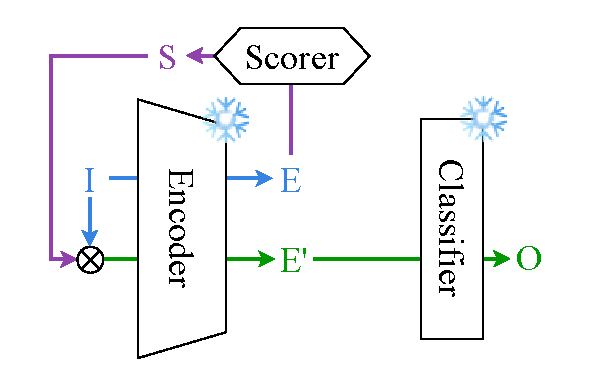
\includegraphics[scale=0.65]{./img/idea.pdf}
    \caption{General idea of the method. Given a traditional classifier (encoder and classification head), we introduce a new module (scorer) that learns to score the input $I$ of the encoder given its embeddings $E$.} \label{fig:training}
\end{figure}

\begin{figure}[t!]
    \centering
    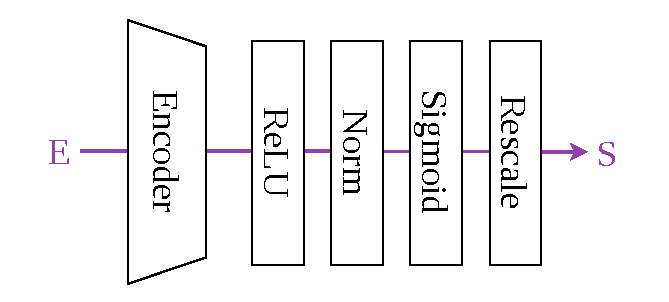
\includegraphics[scale=0.65]{./img/scorer-arch.pdf}
    \caption{Architecture of the scorer} \label{fig:scorer}
\end{figure}

The flow between the encoder and the classifier is as usual. The newly introduced model, called scorer for simplicity, should take as input some information of the input features of the explainee model and it outputs a score for each of them. In case of classifiers, we use the embedding space of the encoder as inputs for the scorer.

We also note that in principle we could provide to the scorer the original input itself. Intuitively, this formulation would still allow to learn some reasonable attribution maps that highlight what is relevant in the input as the goal is still to minimize the task specific loss. However, it would require the scorer to solve the whole classification task as well and no signal from the target model to explain would be included in the flow, so the result of this setup would be closer to an explainable-by-design model.

In terms of architecture, a crucial choice for the scorer, although unusual, is how its output head is designed. A high-level depiction of the architecture is provided in \Cref{fig:scorer}. The scorer itself contains an encoder to refine the input and the output activations it produces are passed through: 
\begin{enumerate*}
    \item a rectified linear unit (ReLU) activation, 
    \item a sigmoid activation, and 
    \item rescaled into $[0, 1]$ . 
\end{enumerate*}
The ReLU activation is used to impose a strong distinction between relevant signal (activation greater than $0$) and background that is not useful for the attribution map. The sigmoid function squeezes the scores into $[0, 1]$ and adds a further level of non-linearity, and the final rescaling actually ensures that the scores span from $0$ to $1$.



\section{Training and Inference}

The scorer module introduced to compute attribution scores is implemented as a neural network and therefore requires training. As we aim at solving the problem defined in \Cref{sec:problem}, we can reformulate it to an optimization problem that can be used to train neural networks. Therefore, we can define the loss function as the following:
\begin{equation}
    \label{eq:loss_naive}
    \begin{aligned}
        \L(\x, \S; f) =\,\, &\L_\text{task}(\x \otimes \S; f) \\
        &+ \gamma_1 \left( \frac{1}{\vert \S \vert} \sum_i^{\vert S \vert} s_i \right)^2 \\
        &+ \gamma_2 \frac{1}{\vert \S \vert} \sum_i^{\vert S \vert} (s_i \cdot (1-s_i))^2 \\
    \end{aligned}
\end{equation} 
where $\L_\text{task}$ is the task-specific loss (cross-entropy in our case), the first penalty term encourages sparsity in the attribution scores so that few positions have high values, and the second penalty term is for pushing scores to be closer to either $0$ or $1$ so that it is more similar to a binary mask. $\gamma_1$ and $\gamma_2$ are instead hyperparameters to weight the importance of the two penalties. 

Ideally, we would like to avoid having to choose and tune arbitrary hyperparameters such as $\gamma_1$ and $\gamma_2$. It turns out that, by how the problem is posed, it is possible to define these two hyperparameters in such a way that they are self-calibrating. We are able to do this by exploiting the information we have about the loss function during training. The idea is to use the inverse distance between the loss evaluated with the masked input and the original one as the weight for the penalties. In this way, the intuition is that when the produced attribution map is preserving the loss, the weight of the penalties can be increased, while if the original loss is not preserved, the penalties are down-weighted so that the learning process can focus on preserving the original capabilities first without being drifted away by the penalties. Therefore, our final training loss is defined as follows:
\begin{equation}
    \label{eq:loss}
    \begin{gathered}
        \begin{aligned}
            \L(\x, \S; f) =\,\, &\L_\text{task}(\x \otimes \S; f) \\
            &+ \gamma \left( \frac{1}{\vert \S \vert} \sum_i^{\vert S \vert} s_i \right)^2 \\
            &+ \gamma \frac{1}{\vert \S \vert} \sum_i^{\vert S \vert} (s_i \cdot (1-s_i))^2 \\
        \end{aligned} \\
        \text{with } \gamma = \texttt{clip}\left\{ \frac{1}{\L_\text{task}(\x \otimes \S; f) - \L_\text{task}(\x; f) + \varepsilon}, [0, 1] \right\},
    \end{gathered}
\end{equation}
where $\gamma$ is the self-calibrating weight based on the distance between losses and $\texttt{clip}$ constrains the weight in $[0, 1]$ to avoid having values that grow uncontrollably, which would make the penalties reach unreasonably high magnitudes, or that go below zero, which would have the opposite effect we aim at achieving.

In terms of parameter updates, we must note that this method does not require to modify the target model as its weights are kept frozen when training the scorer, as depicted in \Cref{fig:training}. This avoids leaking any relevant information for the scorer into the original classifier, so that we can ensure that what it learns is to actually provide attribution maps for the target model without any shortcut. 

\begin{figure}[t!]
    \centering
    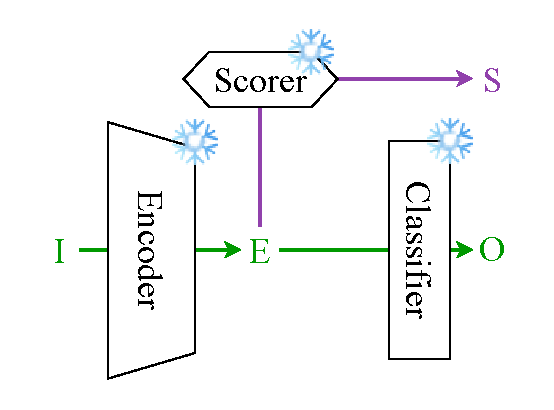
\includegraphics[scale=0.65]{./img/inference.pdf}
    \caption{At inference time, the flow of the classifier is unaffected by the scorer. The output of the scorer corresponds to the attribution map.} \label{fig:inference}
\end{figure}

At inference time, as depicted in \Cref{fig:inference}, this method works transparently alongside the existing classification model. It does not disrupt any of its normal flow and only uses some intermediate information provided by the encoder that is fed into the scorer to determine the output attribution scores.


\subsection{Text Modality} \label{sec:text_scorer}

For text classification, we consider the standard approach based on tokenizing the text sequence and mapping it to embeddings \cite{text_survey_2022}. The flow of the classification model is therefore the following:
\begin{enumerate*}
    \item split sentence into tokens according to a vocabulary,
    \item embed each token based on some static embeddings,
    \item refine the initial embeddings through the text encoder,
    \item pool the resulting embeddings and pass through the classifier.
\end{enumerate*}
The embeddings at step (c) are the most information rich and can be used as the input of the scorer that produces a score for each input token. At training time, as depicted in \Cref{fig:training_text}, we apply these scores to weigh the static embeddings at step (b) before passing them through the encoder. This choice is motivated by two aspects: on the one hand, as we need to integrate the learned attribution maps into the training process, we have to apply the scores at some stage where the input is differentiable and, as the input tokens are discrete and non-differentiable, the first layer at which this is possible is after applying the static embeddings. On the other hand, applying the learned attribution maps on the embeddings produced by the final text encoder would have the risk of being ineffective as each token already had the opportunity to interact with each other first which would make masking an embedding not the same as masking an input token. 

\begin{figure}[t!]
    \begin{subfigure}[b]{0.49\textwidth}
        \centering
        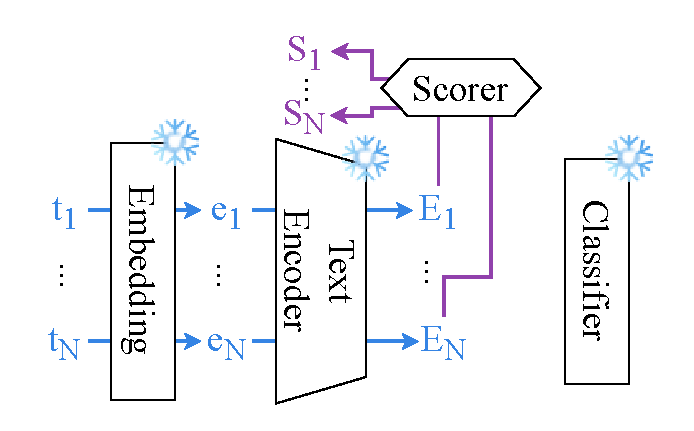
\includegraphics[scale=0.6]{./img/arch-text1.pdf}
        \caption{}
    \end{subfigure}
    \quad
    \begin{subfigure}[b]{0.49\textwidth}
        \centering
        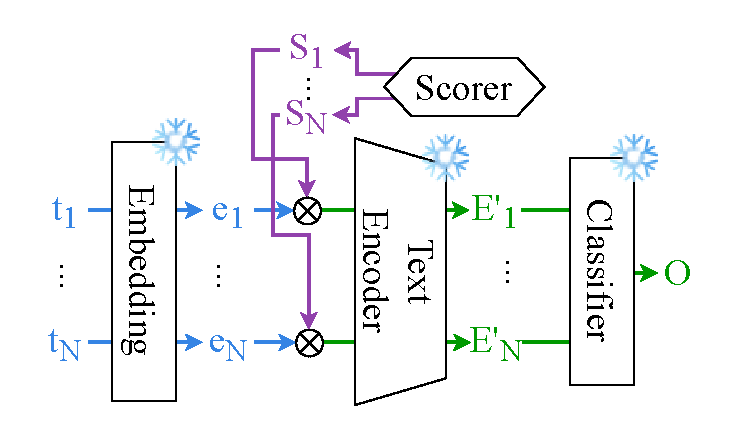
\includegraphics[scale=0.6]{./img/arch-text2.pdf}
        \caption{}
    \end{subfigure}
    \caption{Training architecture for text classifiers} \label{fig:training_text}
\end{figure}



\subsection{Image Modality} \label{sec:image_scorer}

\begin{figure}[t!]
    \centering
    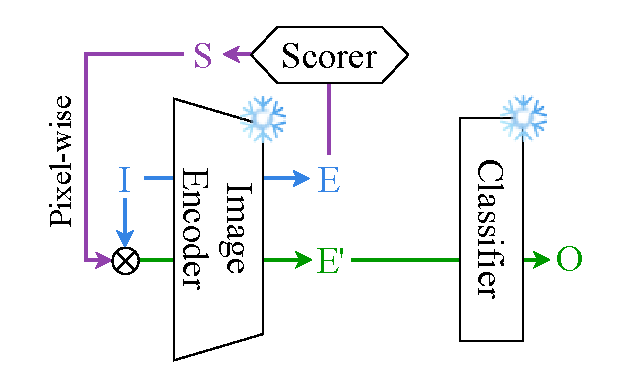
\includegraphics[scale=0.65]{./img/arch-image.pdf}
    \caption{Training architecture for image classifiers} \label{fig:training_image}
\end{figure}

For image classification, we use the traditional approach consisting of an image encoder with a classification head \cite{image_survey_2022}. The flow of the classification model is therefore the following:
\begin{enumerate*}
    \item embed the input image with the encoder,
    \item pool the resulting embeddings and pass through the classifier.
\end{enumerate*}
The embeddings at step (a) can be used as the input of the scorer that produces a score for each input pixel. At training time, as depicted in \Cref{fig:training_image}, we apply these scores to weigh each pixel of the input image before passing them through the encoder. Differently from text, in this case we do not need to add any additional considerations as the input image is already differentiable and the whole process can be directly integrated into the training process.


\subsection{Multimodality}

\begin{figure}[t!]
    \centering
    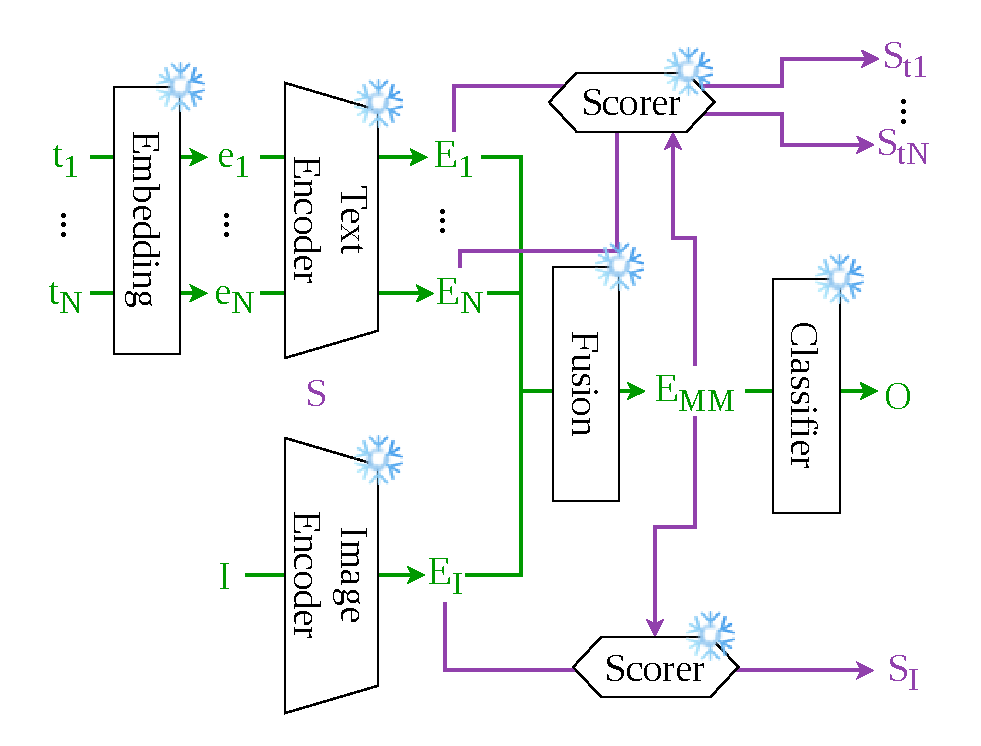
\includegraphics[scale=0.6]{./img/arch-multi.pdf}
    \caption{Inference for text-image classifiers} \label{fig:inference_multi}
\end{figure}

When moving to multimodal models, we can naturally extend our idea by combining the two scorers for text and image as we described in \Cref{sec:text_scorer,sec:image_scorer}. We depict this idea in \Cref{fig:inference_multi} for the case of text-image models. Additionally, in the case of multimodal models, the output of the two encoders are merged through a fusion layer \cite{fusion}, which stays frozen as the rest of the classifier. To avoid losing cross-modality information, the scorers in the multimodal case also take, alongside the embeddings of their modality, the output produced by the fusion layer as conditioning. The loss function is also modified to account for the two scorers: firstly, by extending \Cref{eq:loss} to the multimodal case, we evaluate the cross-entropy loss with both text and image masked so that the scorers are encouraged to preserve the original model. Secondly, to make the task easier and guide the learning process, we also minimize the cross-entropy of the two modalities separately by masking only either the text or the image. Thirdly, as there are two scorers, we introduce two sets of penalties to also handle the attribution maps produced by the two modalities separately. Therefore, after training the target multimodal classifier, we keep both encoders, the fusion layer, and the classification head frozen. Then, we train the two scorers by optimizing the following function:
\begin{equation}
    \begin{gathered}
        \begin{aligned}
            \L(\x_1|\x_2, \S_1|\S_2; f) =\,\, 
            & \L_\text{task}(\x_1 \otimes \S_1 | \x_2 \otimes \S_2; f) \\
            &+ \L_\text{task}(\x_1 \otimes \S_1 | \x_2; f) + \L_\text{task}(\x_1 | \x_2 \otimes \S_2 ; f)\\
            &+ \gamma \left( \frac{1}{\vert \S_1 \vert} \sum_i^{\vert S_1 \vert} s_{1,i} \right)^2 
             + \gamma \left( \frac{1}{\vert \S_2 \vert} \sum_j^{\vert S_2 \vert} s_{2,j} \right)^2 \\
            &+ \gamma \frac{1}{\vert \S_1 \vert} \sum_i^{\vert S_1 \vert} (s_{1,i} \cdot (1-s_{1,i}))^2
             + \gamma \frac{1}{\vert \S_2 \vert} \sum_j^{\vert S_2 \vert} (s_{2,j} \cdot (1-s_{2,j}))^2 \\
        \end{aligned} \\
        \text{with } \gamma = \frac{1}{\texttt{clip}\{ \L_\text{task}(\x_1 \otimes \S_1 | \x_2 \otimes \S_2; f) - \L_\text{task}(\x_1|\x_2; f), [0, 1] \}},
    \end{gathered}
\end{equation}
where:
\begin{itemize}
    \item $\x_1$ and $\x_2$ are the inputs of the two modalities,
    \item $\S_1$ and $\S_2$ are the attribution scores of the two modalities,
    \item $\gamma$ is the self-calibrating parameter based on the logits obtained by masking both modalities.
\end{itemize}

    \chapter{Experimental Setup} \label{ch:setup}



\section{Metrics}

It is well-known that evaluating an explainability method is hard and currently there is no consensus on how it should be done \cite{L_fstr_m_2022}. However, it is unfeasible and unreasonable to manually evaluate attribution maps as it is time-consuming and it might not follow human intuition, while still correctly explaining the model. Therefore, on a quantitative side, we adopt a diverse set of commonly used metrics \cite{gevaert2024evaluating} with the goal of covering different aspects and desiderata of an explanation, while recognizing that no metric alone provides a reasonable way to assess an explainability method. More specifically, to assess whether the explanation is faithful to the model, we adopt average drop \cite{gradcam_plusplus} and deletion AUC \cite{deletion_auc}. Conversely, to assess how the explanation is appealing, we use complexity \cite{complexity_metric} and sparsity \cite{sparsity_metric}. In the rest of this section, we present the chosen metrics.


\paragraph{Average drop.}
Average drop \cite{gradcam_plusplus} measures how much the confidence of a model decreases when only the relevant portion of the input is provided. First, the attribution map is used as a multiplicative scale to weight the input and produce its masked version. Then, a comparison is performed between the prediction confidence of the model using the full input and the masked one. More formally, let $f(\cdot)$ denote the model’s confidence score for the predicted class on a given input, $x$ be the original input, and $x_{\text{masked}}$ be the masked input. Average drop is computed as:
\begin{equation}
    \texttt{average drop} = \max\Big\{ 0, f(x) - f(x_{\text{masked}}) \Big\}.
\end{equation}
Lower values indicate that the explanation successfully captures the most relevant regions for the prediction, as the confidence remains high even after masking. Conversely, a high average drop indicates that important information has been removed, which means that the explanation is less faithful.


\paragraph{Deletion AUC}
Deletion Area Under the Curve (deletion AUC) is an extension of average drop and evaluates how quickly a model’s confidence decreases as the most relevant input features are progressively removed \cite{deletion_auc}. Starting from the original input, features are iteratively removed in descending order of attribution importance, and the model’s confidence score is recorded after each removal step. Formally, given the attribution map, the confidence score $f(x_k)$ is computed after removing the top $k$ most relevant features according to the attribution scores. By plotting the confidence scores as a function of the importance levels, we obtain a curve and the metric is computed as the area under it.

A lower deletion AUC indicates that removing highly attributed regions rapidly degrades the model’s confidence, suggesting that the explanation correctly identifies regions critical to the model’s decision. On the other hand, higher deletion AUC indicates that the attribution map is not correctly ranking the most relevant features as they are not associated to the highest values.


\paragraph{Complexity} Complexity evaluates how much of the input space is relevant according to the attribution map \cite{complexity_metric}. This metric provides an idea of how big the relevant region in the attribution map is and can be useful to determine how easily interpretable the map is. In practice, we compute complexity of an attribution map $S$ as its norm to capture its magnitude and therefore how much of the input space is relevant:
\begin{equation}
    \texttt{complexity} = \Vert S \Vert.
\end{equation}

Lower complexity values correspond to more compact explanations, which, intuitively, are generally preferred from a human perspective.


\paragraph{Sparsity} Sparsity measures the extent to which an attribution map is concise and concentrates relevance on a small subset of the input features \cite{sparsity_metric}. Formally, given an attribution score $S$, sparsity is computed as:
\begin{equation}
    \texttt{sparsity} = \frac{S_\text{max}}{S_\text{mean}},
\end{equation}
where $S_\text{max}$ is the maximum of the attribution map and $S_\text{mean}$ is its mean. It is worth noting that, as we normalize attribution maps into $[0, 1]$, the numerator of the formula is always $1$.

Higher sparsity indicates that the explanation is more concentrated in specific regions, reducing visual clutter and improving interpretability. On the contrary, lower sparsity indicates that many regions of the attribution map are active which might make it more difficult to understand.




\section{Baselines} \label{sec:baselines}

We compare the proposed approach against several other attribution methods. For our benchmarks, we choose well-known approaches for neural networks that work with any type of data format so that we can apply them across different modalities. In particular, we start from simple methods such as Saliency and Guided Backpropagation, and move to more complex ones such as Integrated Gradients, DeepLIFT, and SHAP-based approaches. The rest of this section presents our baselines of choice.

\paragraph{Saliency.} Saliency maps \cite{saliency} are a simple gradient-based explainability baseline for neural networks. The method computes the gradient of the model output with respect to the input features and interprets the magnitude of each partial derivative as an indicator of local sensitivity. Features with larger absolute gradient values are considered more influential as perturbing them would affect the output the most. However, although simple and straightforward, they are often noisy and can suffer from gradient saturation effects, particularly when applied to deep neural networks.

\paragraph{Guided Backpropagation.}
Guided Backpropagation \cite{guided_backprop} is a heuristic approach that modifies the standard backpropagation procedure by suppressing negative gradients during the backward pass so that only gradients corresponding to positive forward and backward signals are propagated. This allows to produce sharper and visually clearer saliency maps. However, this approach lacks a rigorous theoretical foundation. It cannot be proved that it satisfies any desirable property and it may not faithfully reflect the underlying process of the model.

\paragraph{Integrated Gradients.}
Integrated Gradients (IG) \cite{lig} is a method based on integrating the gradient along a continuous path from a baseline input $x'$ to the actual input $x$. Formally, the attribution for a feature $i$ is defined as:
\begin{equation}
    \texttt{IG}_i(x) = (x_i - x'_i) \int_{0}^{1} 
    \frac{\partial f\big(x' + \alpha (x - x')\big)}{\partial x_i} 
    \, d\alpha.
\end{equation}
Formulated in this way, Integrated Gradients has some theoretical guarantees and satisfies the axioms of sensitivity (i.e., the attribution should be different given two inputs differing by one feature but with different labels) and implementation invariance (i.e., the attribution should be identical for functionally equivalent models).
In practice, the integral is approximated numerically using a finite Riemann sum, which introduces a trade-off between computational cost and approximation accuracy. Overall, Integrated Gradients is generally more stable and less prone to saturation, although its results depend on the choice of baselines.

\paragraph{DeepLIFT.}
Deep Learning Important FeaTures (DeepLIFT) \cite{deeplift} explains predictions by comparing neuron activations to those obtained from a reference input. It propagates activation differences backward through the network using specific contribution rules. For each neuron, the deviation from its reference activation is decomposed and attributed to its inputs. In practice, DeepLIFT mitigates issues related to saturation and flat activation regions. Moreover, it satisfies a summation-to-delta property, ensuring that the total attributions equal the difference between the model output at the input and at the reference. However, similar to Integrated Gradients, the method depends on the selection of an appropriate reference input, which can influence the resulting explanations.

\paragraph{DeepLIFT-SHAP.}
DeepLIFT-SHAP \cite{deepliftshap} uses DeepLIFT as a way to approximate SHAP (SHapley Additive exPlanations) values \cite{deepliftshap,shap}. SHAP is grounded in the concept of Shapley values from cooperative game theory \cite{shapley_values}. It sees each feature as a player in a cooperative game, and its contribution to the prediction corresponds to its average marginal contribution across all possible feature subsets. Due to its computational complexity, Shapley values have to be approximated. DeepLIFT-SHAP computes them efficiently by applying DeepLIFT across multiple reference baselines and averaging the resulting attributions. This preserves the additive structure of SHAP while remaining computationally feasible for deep neural networks.

\paragraph{Gradient-SHAP.}
Gradient-SHAP \cite{gradient_shap} is another approach for approximating SHAP values by applying integrated gradients through stochastic sampling of baselines. Rather than integrating along a single deterministic path from a given baseline, the method samples random interpolation points between reference samples and the input. By averaging gradients computed along these sampled paths, Gradient-SHAP is able to approximate Shapley value attributions. Moreover, this stochastic formulation improves robustness to local irregularities in the gradient landscape. However, computational complexity increases with the number of samples required to obtain stable estimates.



\begin{table}[t!]
    \centering
    \footnotesize
    \def\arraystretch{0.9}
    \caption{Datasets used for evaluation} \label{tab:datasets}
    \begin{tabular}{llp{7cm}}
        \toprule
        \textbf{Modality} & \textbf{Name} & \textbf{Task} \\
        \midrule
        \multirow{3}{*}{Text} & Tweet Sentiment Extraction & Sentiment analysis, short texts. \\ 
                              & IMDB                       & Sentiment analysis, long texts. \\
                              & LIAR                       & Fact checking. \\
        \midrule
        \multirow{3}{*}{Image} & MNIST      & Image classification, grayscale low-resolution. \\ 
                               & CIFAR-10   & Image classification, colored low-resolution. \\ 
                               & Imagenette & Image classification, colored high-resolution. \\ 
        \midrule
        \multirow{3}{*}{Multimodal} & Flickr8k & Image-caption alignment. \\ 
                                    & Hateful Memes & Hateful content detection. \\ 
                                    & SNLI-VE & Visual entailment. \\ 
        \bottomrule
    \end{tabular}
\end{table}

\section{Datasets}

To comprehensively evaluate the proposed attribution methods, we use a diverse collection of datasets spanning text, image, and multimodal tasks with varying degrees of complexity. In particular, the datasets range from short to long texts, from low-resolution to high-quality images, and from simple discriminative tasks to more complex reasoning ones. In this section, we present all the datasets we use for evaluation and, in \Cref{tab:datasets}, we provide a summary of these datasets.



\subsection{Text Classification}

For the textual modality, we consider Tweet Sentiment Extraction \cite{tweet_sentiment,mteb}, IMDB \cite{imdb}, and LIAR \cite{politifact} so that we cover different domains, linguistic styles, and document lengths. 

\paragraph{Tweet Sentiment Extraction.}
Tweet Sentiment Extraction \cite{tweet_sentiment,mteb} consists of short, informal social media posts annotated with binary sentiment labels. This dataset was selected as social media posts are typically concise and contain non-standard language such as abbreviations, hashtags, emojis, and typos. This high lexical variability and limited context make this dataset particularly suitable for studying fine-grained token-level attributions, as relevant sentiment cues may be sparse and embedded within noisy text.

\paragraph{IMDB.}
The IMDB movie reviews dataset \cite{imdb} is a large-scale binary sentiment classification benchmark composed of long-form movie reviews. In contrast to short tweets, reviews often contain multiple arguments, narrative elements, and mixed sentiment expressions. This dataset allows evaluating attribution methods under long-context conditions, where relevant evidence may be distributed across the document. 

\paragraph{LIAR.}
The LIAR benchmark \cite{politifact} is composed of political statements extracted from PolitiFact, a fact checking website, where each document is associated with a binary label according to their factual correctness. This dataset provides a more reasoning-intensive setting compared to IMDB while maintaining a setup with longer documents to make the task more challenging and more interesting from an explainability perspective.


\subsection{Image Classification}

To evaluate attribution in the visual domain, we use MNIST \cite{mnist}, CIFAR-10 \cite{cifar10}, and Imagenette \cite{imagenette}, three standard computer vision benchmarks with increasing visual and semantic complexity.

\paragraph{MNIST.}
MNIST \cite{mnist} is a dataset consisting of grayscale images of size $28 \times 28$ containing handwritten digits. It is a dataset with a simple visual structure and limited background variation, which makes it a good baseline to check the effectiveness of explainability methods in the easiest scenario.

\paragraph{CIFAR-10.}
CIFAR-10 \cite{cifar10} contains $32 \times 32$ color images distributed across ten object categories. Compared to MNIST, it introduces more intra-class variability, background noise, and color information, which increases the level of difficulty. Therefore, attribution maps in this case should be slightly more challenging to determine due to the presence of more noise.

\paragraph{Imagenette.}
Imagenette \cite{imagenette} is a subset of ImageNet \cite{imagenet} composed of ten easily distinguishable classes. We choose this version due to computational limitations. The images in the dataset are higher in resolution and exhibit richer semantic structure than CIFAR-10, making the task more complex and closer to a real-life application.


\subsection{Multimodal Classification}

To extend our evaluation beyond unimodal settings, we also consider multimodal benchmarks. In particular, we evaluate on Flickr8k \cite{flickr8k}, Hateful memes \cite{memes}, and SNLI-VE \cite{snli_ve}.

\paragraph{Flickr8k.}
Flickr8k \cite{flickr8k} consists of images paired with natural language captions. We formulate a binary classification task in which the model must determine whether a given caption correctly describes the image. This dataset acts as a starting baseline as it provides a simple task of matching text and image, without involving complex semantic connections.

\paragraph{Hateful Memes.}
The Hateful Memes dataset \cite{memes} contains the image and the textual content of memes in which hateful intent often emerges only from the interaction between the two modalities. This makes the task more challenging than Flickr8k as it does not simply require to align the two representations and involves some semantic understanding. This also makes generating attribution maps more interesting to understand how the model is connecting different concepts.

\paragraph{SNLI-VE.}
SNLI-VE \cite{snli_ve} is composed of image-sentence pairs from Stanford Natural Language Inference \cite{snli} and Flickr30k \cite{flickr30k} and it is designed for the task of visual entailment. An image and a short text act as the premise while another short text provides a hypothesis. The task consists of predicting whether there is entailment, contradiction, or neutrality between premise and hypothesis. This dataset requires fine-grained semantic alignment between visual and linguistic content which introduces a further level of difficulty compared to Hateful Memes.



\section{Architectures}


\paragraph{Text.} For text classification, we use two distinct transformer encoders \cite{transformer} for the classifier and the scorer module. For the classification task itself, we use RoBERTa \cite{roberta} as the pretrained encoder. For the scorer module, we instead use a custom small transformer initialized from scratch. It takes as input the embeddings of each token produced by RoBERTa and outputs the attribution scores. During training, these scores are applied to the static embeddings of the input tokens, before passing through the transformer layers of RoBERTa.


\paragraph{Image.} For image classification, we use a vision transformer \cite{vit} for the classification task and a U-Net \cite{unet} like network for the scorer module. The U-Net starts from the final embeddings produced by the vision transformer and upsamples it using transposed convolutions. As in the original U-Net, intermediate layers from the vision transformer are also included during upsampling as skip connections to provide more information. During training, the attribution map produced by the scorer is applied to the input image before feeding it through the backbone.


\paragraph{Text-image.} For multimodal classification, the model is a combination of the text and image classifiers. We therefore use both RoBERTa and vision transformer, and the outputs of the two encoders are put together through a fusion layer, which is implemented as a small transformer encoder. For the scorers, both modules work as previously described with the addition of a further step where the embeddings produced by the fusion model are incorporated into the flow to account for cross-modal information.




\section{Implementation Details}

We use PyTorch \cite{pytorch} to implement our method and to train the neural networks for each task. Pretrained transformers and vision transformers are provided by Hugging Face. All datasets are taken from Hugging Face \cite{huggingface} as well, with the exception of MNIST and CIFAR which are provided by TorchVision \cite{torchvision}. For the baseline explainability methods, we use the implementation provided by Captum \cite{captum}.  

During training, we split the datasets into training, validation, and test sets. We use the default splits provided by the dataset when available, and manually split when the dataset is provided as a whole.
When training the models, we first fine-tune the classifier while keeping the scorer module frozen. Then, we train the scorer by keeping the classifier frozen. We use as optimizer AdamW \cite{adamw} in all cases with a learning rate of $10^{-5}$ for fine-tuning and $2 \cdot 10^{-4}$ for training the scorer. All experiments have been executed on NVIDIA A100 GPUs with 80GB of memory provided by the National Institute of Informatics in Japan. The base classifiers are trained for 10 epochs maximum, while the scorers for 5, as we observed that they tend to stop very early due to early stopping. It took us approximately two hours to train each base classifier and its scorer on a single NVIDIA A100, and an additional hour to evaluate across all baselines.
    \chapter{Results} \label{ch:results}


\section{Text Classification}

Quantitative results for Tweet Sentiment Extraction, IMDB, and LIAR are presented in \Cref{tab:tweet}, \Cref{tab:imdb}, and \Cref{tab:politifact}, respectively. Radar plots of the metrics is also reported in \Cref{fig:radar_text}. In all three datasets, our method yields the lowest complexity score and consistently achieves the second-best sparsity score after Saliency. Instead, Guided Backpropagation is the method that performs best in terms of average drop while DeepLIFT has better results in terms of deletion AUC. Also, as an overall behavior across the three datasets, we can observe that Integrated Gradients, DeepLIFT, DeepLIFT-SHAP, Gradient-SHAP, and Guided Backpropagation all result in high complexity and low sparsity. Saliency instead is the worst performing in terms of average drop and deletion AUC, but achieves the best sparsity and reasonable complexity. This highlights a clear trade-off that these methods exhibit between producing attribution maps that are visually appealing and more faithful to the model prediction.

\begin{table}[t!]
    \centering
    \caption{Results for Tweet Sentiment Extraction} \label{tab:tweet}
    \small
    \def\arraystretch{0.75}
    \makebox[\linewidth][c]{%
    \begin{tabular}{lcccc}
        \toprule
        \textbf{Method} & \textbf{Average drop $\downarrow$} & \textbf{Deletion AUC $\downarrow$} & \textbf{Complexity $\downarrow$} & \textbf{Sparsity $\uparrow$} \\
        \midrule
        Saliency         & 1.91 \std{1.76}          & 2.49 \std{1.78}          & 13.11  \std{3.02}          & \textbf{412.95 \std{158.54}} \\
        Guided Backprop. & \textbf{0.09 \std{0.19}} & \textbf{1.38 \std{0.98}} & 312.17 \std{33.18}         & 2.03   \std{0.23} \\
        Int. Gradients   & 0.20 \std{0.57}          & 1.68 \std{1.43}          & 279.29 \std{107.56}        & 2.80   \std{1.90} \\
        DeepLIFT         & 0.42 \std{0.86}          & 1.47 \std{1.25}          & 311.62 \std{101.81}        & 2.31   \std{1.04} \\
        DeepLIFT-SHAP    & 0.44 \std{0.90}          & 1.43 \std{1.19}          & 311.00 \std{87.70}         & 2.22   \std{0.83} \\
        Gradient-SHAP    & 0.34 \std{0.82}          & 1.43 \std{1.22}          & 298.72 \std{99.06}         & 2.40   \std{1.00} \\
        Ours             & 1.11 \std{1.52}          & 1.61 \std{1.57}          & \textbf{2.71   \std{1.04}} & 87.21  \std{72.40} \\
        \bottomrule
    \end{tabular}
    }
\end{table}

\begin{table}[t!]
    \centering
    \caption{Results for IMDB} \label{tab:imdb}
    \small
    \def\arraystretch{0.75}
    \makebox[\linewidth][c]{%
    \begin{tabular}{lcccc}
        \toprule
        \textbf{Method} & \textbf{Average drop $\downarrow$} & \textbf{Deletion AUC $\downarrow$} & \textbf{Complexity $\downarrow$} & \textbf{Sparsity $\uparrow$} \\
        \midrule
        Saliency         & 3.19 \std{1.04}          & 3.06 \std{0.99}          & 18.57  \std{5.97}            & \textbf{114.05 \std{91.08}} \\
        Guided Backprop. & \textbf{0.05 \std{0.14}} & 1.62 \std{0.56}          & 313.09 \std{41.16}           & 2.04   \std{0.29} \\
        Int. Gradients   & 0.72 \std{1.39}          & 1.76 \std{1.06}          & 279.72 \std{171.69}          & 4.37   \std{4.96} \\
        DeepLIFT         & 0.15 \std{0.63}          & 1.61 \std{0.81}          & 315.50 \std{108.50}          & 2.35   \std{1.23} \\
        DeepLIFT-SHAP    & 0.14 \std{0.63}          & \textbf{1.58 \std{0.78}} & 315.62 \std{103.78}          & 2.32   \std{1.20} \\
        Gradient-SHAP    & 0.10 \std{0.50}          & 1.66 \std{0.81}          & 296.16 \std{111.63}          & 2.52   \std{1.24} \\
        Ours             & 0.46 \std{0.63}          & 1.83 \std{0.76}          & \textbf{4.90   \std{2.22}}   & 12.64  \std{12.29} \\
        \bottomrule
    \end{tabular}
    }
\end{table}

\begin{table}[t!]
    \centering
    \caption{Results for LIAR} \label{tab:politifact}
    \small
    \def\arraystretch{0.75}
    \makebox[\linewidth][c]{%
    \begin{tabular}{lcccc}
        \toprule
        \textbf{Method} & \textbf{Average drop $\downarrow$} & \textbf{Deletion AUC $\downarrow$} & \textbf{Complexity $\downarrow$} & \textbf{Sparsity $\uparrow$} \\
        \midrule
        Saliency         & 1.44 \std{1.20}          & 1.36 \std{1.14}          & 16.59  \std{5.93}            & \textbf{104.42 \std{85.75}} \\
        Guided Backprop. & \textbf{0.09 \std{0.16}} & 0.74 \std{0.61}          & 316.11 \std{46.54}           & 2.03   \std{0.32} \\
        Int. Gradients   & 0.23 \std{0.61}          & 0.85 \std{0.81}          & 278.28 \std{109.90}          & 2.75   \std{1.50} \\
        DeepLIFT         & 0.21 \std{0.52}          & \textbf{0.72 \std{0.68}} & 323.70 \std{123.19}          & 2.36   \std{1.26} \\
        DeepLIFT-SHAP    & 0.20 \std{0.54}          & 0.73 \std{0.68}          & 323.81 \std{116.52}          & 2.31   \std{1.23} \\
        Gradient-SHAP    & 0.17 \std{0.49}          & 0.73 \std{0.68}          & 312.24 \std{119.44}          & 2.52   \std{1.73} \\
        Ours             & 0.26 \std{0.29}          & 1.00 \std{0.80}          & \textbf{7.71   \std{0.34}}   & 3.08   \std{1.63} \\
        \bottomrule
    \end{tabular}
    }
\end{table}

\begin{figure}[t!]
    \centering
    \begin{subfigure}[c]{0.26\linewidth}
        \centering
        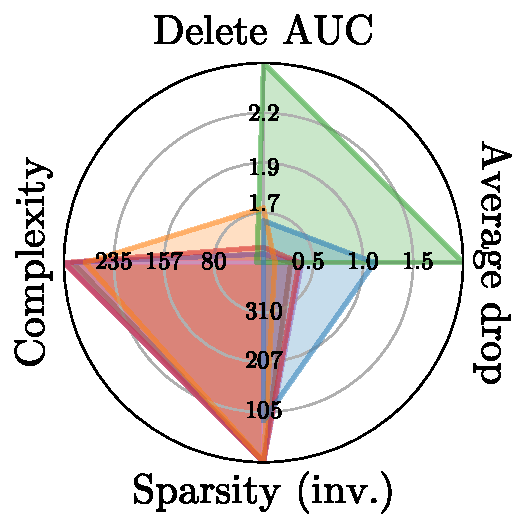
\includegraphics[scale=0.4]{./img/radar-tweet.pdf}
        \caption{Tweet Sentiment}
    \end{subfigure}
    \begin{subfigure}[c]{0.26\linewidth}
        \centering
        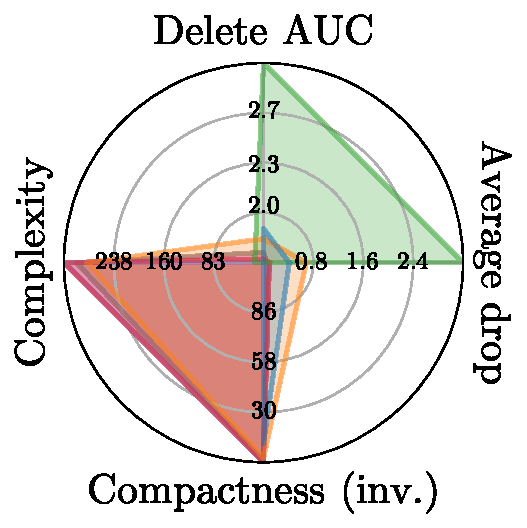
\includegraphics[scale=0.4]{./img/radar-imdb.pdf}
        \caption{IMDB}
    \end{subfigure}
    \begin{subfigure}[c]{0.26\linewidth}
        \centering
        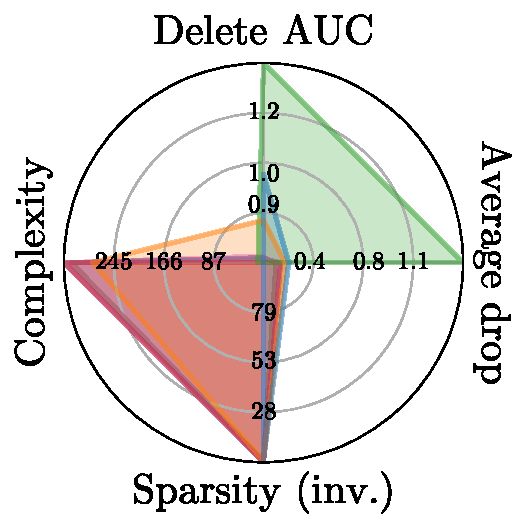
\includegraphics[scale=0.4]{./img/radar-politifact.pdf}
        \caption{LIAR}
    \end{subfigure}
    \begin{subfigure}[c]{0.16\linewidth}
        \centering
        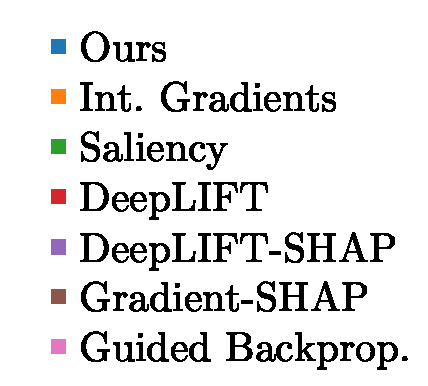
\includegraphics[scale=0.4]{./img/radar-legend.pdf}
    \end{subfigure}
    \caption{Radar plot of the quantitative metrics for the text tasks. The closer to the center, the better.} \label{fig:radar_text}
\end{figure}

Qualitatively, we manually evaluate some samples from IMDB. We choose this dataset as it has longer documents compared to Tweet Sentiment Extraction and its classifier achieves near perfect results, which should make it easier to intuitively evaluate the attribution maps. We selected 100 random samples from the dataset and evaluated them. The main pattern we observed is that our method, compared to the other baselines, has a more decisive scoring system as it favors either very high or very low scores, while the other methods tend to give some degree of importance to each token. Also, we observed that the attribution scores correctly highlight the most relevant terms to decide the sentiment, although it frequently also highlights surrounding terms which are not necessarily relevant according to human intuition. We report in \Cref{fig:imdb_sample} a sample extracted from the dataset. Moreover, in line with the metrics, Integrated Gradients, DeepLIFT, DeepLIFT-SHAP, Gradient-SHAP, and Guided Backpropagation are the methods that produce attribution maps that span across the whole input the most, while Saliency is the method where the scores are more concentrated on a few words.

\begin{figure}[t!]
    \scriptsize
    \centering
    \makebox[\linewidth][c]{%
    \begin{tabular}{lc}
    \textbf{Ours} & {\tt\colorbox[RGB]{221, 62, 42}{\textcolor{black}{\vphantom{Tg}This}} \colorbox[RGB]{249, 132, 85}{\textcolor{black}{\vphantom{Tg}is}} \colorbox[RGB]{217, 52, 34}{\textcolor{black}{\vphantom{Tg}a}} \colorbox[RGB]{190, 15, 10}{\textcolor{white}{\vphantom{Tg}great}} \colorbox[RGB]{207, 38, 24}{\textcolor{white}{\vphantom{Tg}movie.}} \colorbox[RGB]{253, 220, 175}{\textcolor{black}{\vphantom{Tg}Too}} \colorbox[RGB]{255, 243, 226}{\textcolor{black}{\vphantom{Tg}bad}} \colorbox[RGB]{253, 168, 114}{\textcolor{black}{\vphantom{Tg}it}} \colorbox[RGB]{253, 171, 117}{\textcolor{black}{\vphantom{Tg}is}} \colorbox[RGB]{254, 224, 183}{\textcolor{black}{\vphantom{Tg}not}} \colorbox[RGB]{255, 244, 228}{\textcolor{black}{\vphantom{Tg}available}} \colorbox[RGB]{255, 247, 235}{\textcolor{black}{\vphantom{Tg}on}} \colorbox[RGB]{255, 243, 227}{\textcolor{black}{\vphantom{Tg}home}} \colorbox[RGB]{252, 149, 96}{\textcolor{black}{\vphantom{Tg}video.</s>}}}\\
    \textbf{Saliency} & {\tt\colorbox[RGB]{253, 171, 117}{\textcolor{black}{\vphantom{Tg}This}} \colorbox[RGB]{253, 199, 145}{\textcolor{black}{\vphantom{Tg}is}} \colorbox[RGB]{253, 190, 135}{\textcolor{black}{\vphantom{Tg}a}} \colorbox[RGB]{127, 0, 0}{\textcolor{white}{\vphantom{Tg}great}} \colorbox[RGB]{236, 95, 67}{\textcolor{black}{\vphantom{Tg}movie.}} \colorbox[RGB]{253, 197, 142}{\textcolor{black}{\vphantom{Tg}Too}} \colorbox[RGB]{253, 191, 137}{\textcolor{black}{\vphantom{Tg}bad}} \colorbox[RGB]{253, 208, 154}{\textcolor{black}{\vphantom{Tg}it}} \colorbox[RGB]{253, 221, 177}{\textcolor{black}{\vphantom{Tg}is}} \colorbox[RGB]{253, 216, 167}{\textcolor{black}{\vphantom{Tg}not}} \colorbox[RGB]{253, 165, 111}{\textcolor{black}{\vphantom{Tg}available}} \colorbox[RGB]{253, 216, 167}{\textcolor{black}{\vphantom{Tg}on}} \colorbox[RGB]{252, 160, 107}{\textcolor{black}{\vphantom{Tg}home}} \colorbox[RGB]{253, 181, 126}{\textcolor{black}{\vphantom{Tg}video.</s>}}}\\
    \textbf{Guided backprop} & {\tt\colorbox[RGB]{252, 152, 99}{\textcolor{black}{\vphantom{Tg}This}} \colorbox[RGB]{227, 75, 52}{\textcolor{black}{\vphantom{Tg}is}} \colorbox[RGB]{188, 12, 8}{\textcolor{white}{\vphantom{Tg}a}} \colorbox[RGB]{253, 186, 131}{\textcolor{black}{\vphantom{Tg}great}} \colorbox[RGB]{253, 213, 160}{\textcolor{black}{\vphantom{Tg}movie.}} \colorbox[RGB]{253, 199, 145}{\textcolor{black}{\vphantom{Tg}Too}} \colorbox[RGB]{239, 101, 72}{\textcolor{black}{\vphantom{Tg}bad}} \colorbox[RGB]{252, 163, 110}{\textcolor{black}{\vphantom{Tg}it}} \colorbox[RGB]{202, 30, 20}{\textcolor{white}{\vphantom{Tg}is}} \colorbox[RGB]{215, 48, 31}{\textcolor{black}{\vphantom{Tg}not}} \colorbox[RGB]{179, 0, 0}{\textcolor{white}{\vphantom{Tg}available}} \colorbox[RGB]{244, 117, 79}{\textcolor{black}{\vphantom{Tg}on}} \colorbox[RGB]{127, 0, 0}{\textcolor{white}{\vphantom{Tg}home}} \colorbox[RGB]{253, 175, 121}{\textcolor{black}{\vphantom{Tg}video.</s>}}}\\
    \textbf{Int. Gradients} & {\tt\colorbox[RGB]{142, 0, 0}{\textcolor{white}{\vphantom{Tg}This}} \colorbox[RGB]{250, 134, 86}{\textcolor{black}{\vphantom{Tg}is}} \colorbox[RGB]{249, 130, 84}{\textcolor{black}{\vphantom{Tg}a}} \colorbox[RGB]{127, 0, 0}{\textcolor{white}{\vphantom{Tg}great}} \colorbox[RGB]{229, 80, 56}{\textcolor{black}{\vphantom{Tg}movie.}} \colorbox[RGB]{226, 72, 49}{\textcolor{black}{\vphantom{Tg}Too}} \colorbox[RGB]{248, 129, 84}{\textcolor{black}{\vphantom{Tg}bad}} \colorbox[RGB]{251, 139, 88}{\textcolor{black}{\vphantom{Tg}it}} \colorbox[RGB]{253, 175, 121}{\textcolor{black}{\vphantom{Tg}is}} \colorbox[RGB]{255, 247, 236}{\textcolor{black}{\vphantom{Tg}not}} \colorbox[RGB]{253, 171, 117}{\textcolor{black}{\vphantom{Tg}available}} \colorbox[RGB]{252, 149, 96}{\textcolor{black}{\vphantom{Tg}on}} \colorbox[RGB]{232, 85, 60}{\textcolor{black}{\vphantom{Tg}home}} \colorbox[RGB]{244, 118, 79}{\textcolor{black}{\vphantom{Tg}video.</s>}}}\\
    \textbf{DeepLIFT} & {\tt\colorbox[RGB]{249, 130, 84}{\textcolor{black}{\vphantom{Tg}This}} \colorbox[RGB]{239, 101, 72}{\textcolor{black}{\vphantom{Tg}is}} \colorbox[RGB]{237, 97, 69}{\textcolor{black}{\vphantom{Tg}a}} \colorbox[RGB]{253, 194, 139}{\textcolor{black}{\vphantom{Tg}great}} \colorbox[RGB]{252, 140, 89}{\textcolor{black}{\vphantom{Tg}movie.}} \colorbox[RGB]{253, 165, 111}{\textcolor{black}{\vphantom{Tg}Too}} \colorbox[RGB]{240, 105, 74}{\textcolor{black}{\vphantom{Tg}bad}} \colorbox[RGB]{246, 123, 81}{\textcolor{black}{\vphantom{Tg}it}} \colorbox[RGB]{251, 137, 87}{\textcolor{black}{\vphantom{Tg}is}} \colorbox[RGB]{252, 147, 95}{\textcolor{black}{\vphantom{Tg}not}} \colorbox[RGB]{218, 55, 36}{\textcolor{black}{\vphantom{Tg}available}} \colorbox[RGB]{242, 109, 75}{\textcolor{black}{\vphantom{Tg}on}} \colorbox[RGB]{234, 90, 63}{\textcolor{black}{\vphantom{Tg}home}} \colorbox[RGB]{243, 113, 77}{\textcolor{black}{\vphantom{Tg}video.</s>}}}\\
    \textbf{DeepLIFT-SHAP} & {\tt\colorbox[RGB]{248, 129, 84}{\textcolor{black}{\vphantom{Tg}This}} \colorbox[RGB]{242, 109, 75}{\textcolor{black}{\vphantom{Tg}is}} \colorbox[RGB]{241, 108, 75}{\textcolor{black}{\vphantom{Tg}a}} \colorbox[RGB]{253, 194, 139}{\textcolor{black}{\vphantom{Tg}great}} \colorbox[RGB]{252, 140, 89}{\textcolor{black}{\vphantom{Tg}movie.}} \colorbox[RGB]{252, 160, 107}{\textcolor{black}{\vphantom{Tg}Too}} \colorbox[RGB]{230, 82, 57}{\textcolor{black}{\vphantom{Tg}bad}} \colorbox[RGB]{241, 106, 74}{\textcolor{black}{\vphantom{Tg}it}} \colorbox[RGB]{249, 133, 86}{\textcolor{black}{\vphantom{Tg}is}} \colorbox[RGB]{249, 133, 86}{\textcolor{black}{\vphantom{Tg}not}} \colorbox[RGB]{205, 35, 22}{\textcolor{white}{\vphantom{Tg}available}} \colorbox[RGB]{242, 110, 76}{\textcolor{black}{\vphantom{Tg}on}} \colorbox[RGB]{236, 95, 67}{\textcolor{black}{\vphantom{Tg}home}} \colorbox[RGB]{243, 113, 77}{\textcolor{black}{\vphantom{Tg}video.</s>}}}\\
    \textbf{Gradient-SHAP} & {\tt\colorbox[RGB]{251, 139, 88}{\textcolor{black}{\vphantom{Tg}This}} \colorbox[RGB]{254, 232, 200}{\textcolor{black}{\vphantom{Tg}is}} \colorbox[RGB]{253, 187, 133}{\textcolor{black}{\vphantom{Tg}a}} \colorbox[RGB]{127, 0, 0}{\textcolor{white}{\vphantom{Tg}great}} \colorbox[RGB]{217, 52, 34}{\textcolor{black}{\vphantom{Tg}movie.}} \colorbox[RGB]{248, 129, 84}{\textcolor{black}{\vphantom{Tg}Too}} \colorbox[RGB]{255, 247, 236}{\textcolor{black}{\vphantom{Tg}bad}} \colorbox[RGB]{253, 173, 119}{\textcolor{black}{\vphantom{Tg}it}} \colorbox[RGB]{253, 200, 146}{\textcolor{black}{\vphantom{Tg}is}} \colorbox[RGB]{253, 216, 167}{\textcolor{black}{\vphantom{Tg}not}} \colorbox[RGB]{244, 117, 79}{\textcolor{black}{\vphantom{Tg}available}} \colorbox[RGB]{245, 119, 80}{\textcolor{black}{\vphantom{Tg}on}} \colorbox[RGB]{244, 118, 79}{\textcolor{black}{\vphantom{Tg}home}} \colorbox[RGB]{253, 217, 170}{\textcolor{black}{\vphantom{Tg}video.</s>}}}\\
    \end{tabular}
    }
    \caption{Sample from IMDB} \label{fig:imdb_sample}
\end{figure}

Putting all these observations together, we can conclude that our method, being the one with the least complexity metric and with generally higher sparsity, produces attribution maps that are closer to binary masks, indicating that it gives a clear distinction between what the classifier is considering relevant and what it is not, making its attribution maps generally more appealing. Moreover, by achieving decent average drop and deletion AUC, it shows that it is able to highlight relevant features of the input space, which indicates that it does not lose in faithfulness.



\section{Image Classification}
For the image classification tasks, we report the result for MNIST, CIFAR-10, and Imagenette on \Cref{tab:mnist}, \Cref{tab:cifar10}, and \Cref{tab:imagenette}, respectively, while the radar plots are depicted in \Cref{fig:radar_image}. For these datasets, our method consistently achieves the highest average drop and deletion AUC. In terms of complexity, Integrated Gradients is the method performing the best, while, for sparsity, Saliency has the highest results. Instead, as for the case of text, DeepLIFT, DeepLIFT-SHAP, Gradient-SHAP, and Guided Backpropagation all produce highly complex and weakly compact maps, but achieve high results in terms of average drop and deletion AUC. This highlights again a trade-off between faithfulness and appeal that is present among these methods, and ours is again located as a balanced approach for these two requirements.

\begin{table}[t!]
    \centering
    \caption{Results on MNIST} \label{tab:mnist}
    \small
    \def\arraystretch{0.75}
    \makebox[\linewidth][c]{%
    \begin{tabular}{lcccc}
        \toprule
        \textbf{Method} & \textbf{Average drop $\downarrow$} & \textbf{Deletion AUC $\downarrow$} & \textbf{Complexity $\downarrow$} & \textbf{Sparsity $\uparrow$} \\
        \midrule
        Saliency         & 0.63 \std{0.31}          & 0.81 \std{0.14}          & 13.39  \std{4.57}           & \textbf{42.85 \std{36.35}} \\
        Guided Backprop. & 0.07 \std{0.19}          & 0.45 \std{0.10}          & 112.17 \std{13.22}          & 2.03  \std{0.26} \\
        Int. Gradients   & 0.02 \std{0.09}          & 0.57 \std{0.15}          & \textbf{4.86   \std{1.43}}  & 3.64  \std{1.92} \\
        DeepLIFT         & 0.03 \std{0.13}          & 0.45 \std{0.10}          & 111.46 \std{13.58}          & 2.05  \std{0.27} \\
        DeepLIFT-SHAP    & \textbf{0.01 \std{0.10}} & \textbf{0.44 \std{0.11}} & 111.85 \std{16.12}          & 2.05  \std{0.32} \\
        Gradient-SHAP    & 0.01 \std{0.09}          & \textbf{0.44 \std{0.09}} & 110.89 \std{14.69}          & 2.06  \std{0.29} \\
        Ours              & \textbf{0.01 \std{0.08}} & 0.53 \std{0.26}          & 33.65  \std{15.36}          & 22.20 \std{10.97} \\
        \bottomrule
    \end{tabular}
    }
\end{table}

\begin{table}[t!]
    \centering
    \caption{Results on CIFAR-10} \label{tab:cifar10}
    \small
    \def\arraystretch{0.75}
    \makebox[\linewidth][c]{%
    \begin{tabular}{lcccc}
        \toprule
        \textbf{Method} & \textbf{Average drop $\downarrow$} & \textbf{Deletion AUC $\downarrow$} & \textbf{Complexity $\downarrow$} & \textbf{Sparsity $\uparrow$} \\
        \midrule
        Saliency         & 0.88 \std{0.09}          & 0.83 \std{0.05}          & 12.49  \std{7.20}           & \textbf{63.91 \std{58.92}} \\
        Guided Backprop. & 0.21 \std{0.37}          & 0.48 \std{0.08}          & 111.92 \std{12.76}          & 2.03  \std{0.24} \\
        Int. Gradients   & \textbf{0.03 \std{0.16}} & 0.57 \std{0.13}          & \textbf{5.75   \std{1.57}}  & 2.84  \std{1.01} \\
        DeepLIFT         & 0.07 \std{0.22}          & \textbf{0.46 \std{0.09}} & 112.75 \std{16.48}          & 2.04  \std{0.32} \\
        DeepLIFT-SHAP    & 0.06 \std{0.21}          & \textbf{0.46 \std{0.09}} & 113.32 \std{16.49}          & 2.02  \std{0.31} \\
        Gradient-SHAP    & 0.05 \std{0.20}          & 0.48 \std{0.08}          & 111.75 \std{13.80}          & 2.04  \std{0.26} \\
        Ours              & \textbf{0.03 \std{0.15}} & 0.52 \std{0.18}          & 68.44  \std{18.32}          & 5.02  \std{2.01} \\
        \bottomrule
    \end{tabular}
    }
\end{table}

\begin{table}[t!]
    \centering
    \caption{Results on Imagenette} \label{tab:imagenette}
    \small
    \def\arraystretch{0.75}
    \makebox[\linewidth][c]{%
    \begin{tabular}{lcccc}
        \toprule
        \textbf{Method} & \textbf{Average drop $\downarrow$} & \textbf{Deletion AUC $\downarrow$} & \textbf{Complexity $\downarrow$} & \textbf{Sparsity $\uparrow$} \\
        \midrule
        Saliency         & 0.50 \std{0.17}          & 0.53 \std{0.09}          & 10.46  \std{5.07}           & \textbf{73.55 \std{60.17}} \\
        Guided Backprop. & 0.05 \std{0.11}          & 0.28 \std{0.06}          & 112.95 \std{12.52}          & 2.01  \std{0.23} \\
        Int. Gradients   & \textbf{0.01 \std{0.06}} & 0.31 \std{0.11}          & \textbf{5.79   \std{1.76}}  & 2.87  \std{1.20} \\
        DeepLIFT         & \textbf{0.01 \std{0.07}} & 0.28 \std{0.06}          & 112.46 \std{15.83}          & 2.04  \std{0.32} \\
        DeepLIFT-SHAP    & \textbf{0.01 \std{0.07}} & 0.28 \std{0.06}          & 112.46 \std{16.02}          & 2.04  \std{0.31} \\
        Gradient-SHAP    & \textbf{0.01 \std{0.06}} & 0.28 \std{0.06}          & 110.71 \std{14.36}          & 2.06  \std{0.29} \\
        Ours              & 0.02 \std{0.07}          & \textbf{0.27 \std{0.12}} & 60.43  \std{19.45}          & 7.02  \std{2.92} \\
        \bottomrule
    \end{tabular}
    }
\end{table}

\begin{figure}[t!]
    \centering
    \begin{subfigure}[c]{0.26\linewidth}
        \centering
        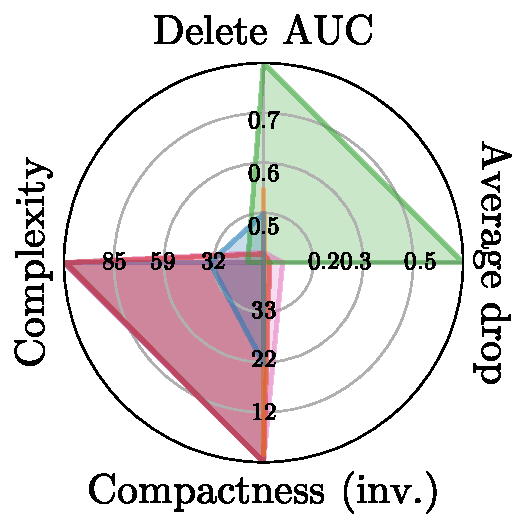
\includegraphics[scale=0.4]{./img/radar-mnist.pdf}
        \caption{MNIST}
    \end{subfigure}
    \begin{subfigure}[c]{0.26\linewidth}
        \centering
        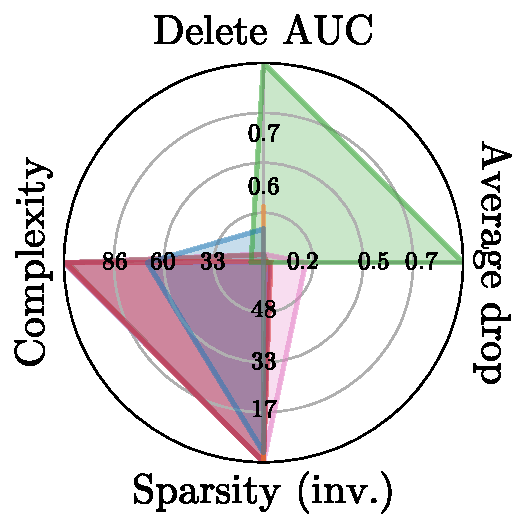
\includegraphics[scale=0.4]{./img/radar-cifar10.pdf}
        \caption{CIFAR-10}
    \end{subfigure}
    \begin{subfigure}[c]{0.26\linewidth}
        \centering
        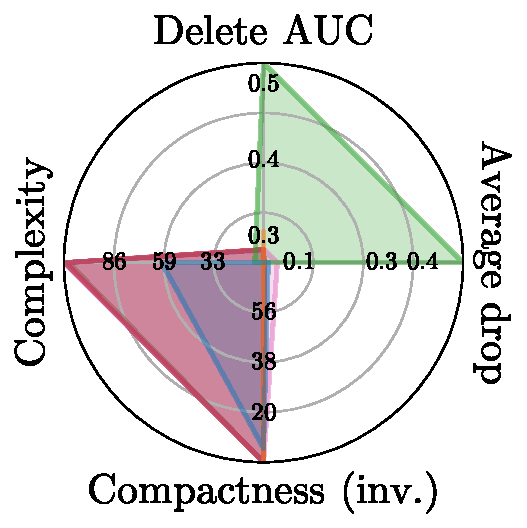
\includegraphics[scale=0.4]{./img/radar-imagenette.pdf}
        \caption{Imagenette}
    \end{subfigure}
    \begin{subfigure}[c]{0.16\linewidth}
        \centering
        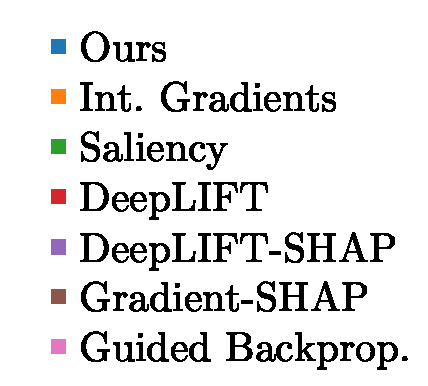
\includegraphics[scale=0.4]{./img/radar-legend.pdf}
    \end{subfigure}
    \caption{Radar plot of the quantitative metrics for the image tasks. The closer to the center, the better.} \label{fig:radar_image}
\end{figure}

Qualitatively, we evaluate 100 random samples from Imagenette. In the case of images, all classifiers have strong performance, therefore, we choose to analyze Imagenette as it contains images of higher resolution. Similarly to the results we obtained for text, we can observe that compared to the other baselines, except Saliency, the attribution map produced with our method is closer to a binary mask with values closer to either $0$ or $1$. Also, compared to gradient-based methods, in the case of images, we can observe that almost all, but Integrated Gradients, produce results that are very focused on a small subset of pixels, which makes results less visually appealing, although performing well in terms of average drop and deletion AUC. Finally, semantically, we observed that almost all attribution maps correctly identify the object of interest in the image by either highlighting it wholly or by identifying key characteristics. We report a sample from the dataset in \Cref{fig:imagenette_sample}.

\begin{figure}[t!]
    \centering
    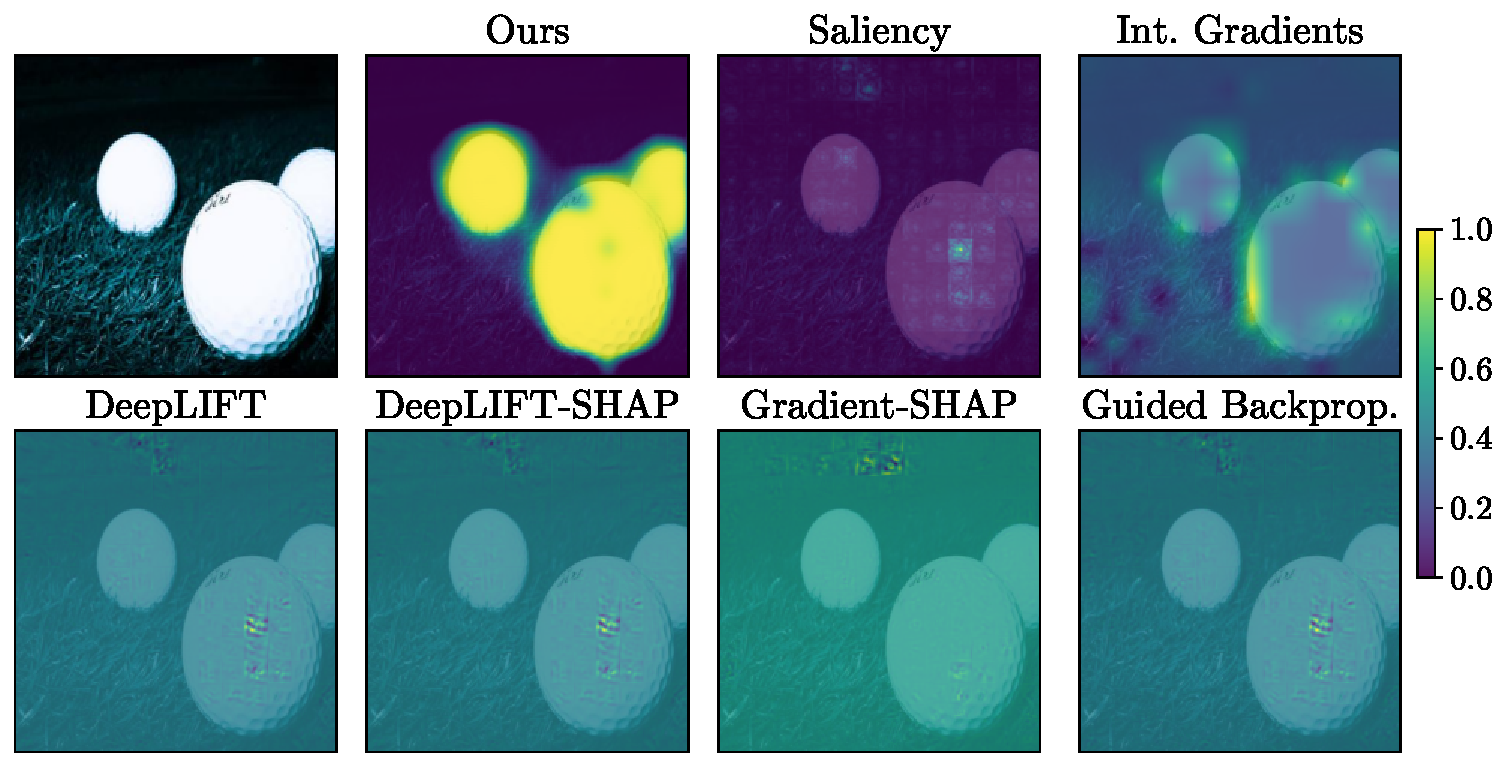
\includegraphics[width=0.9\linewidth]{./img/imagenette.pdf}
    \caption{Sample from Imagenette} \label{fig:imagenette_sample}
\end{figure}

Overall, results with images highlight that, as for text, the attribution maps produced by our method have a clear separation between what is relevant and what is not while also achieving competitive values of average drop and deletion AUC. This again highlights a trade-off between attribution map faithfulness and visual plausibility, and our method is located in the middle ground between the two requirements.



\section{Multimodal Classification}

Results on multimodal datasets are reported in \Cref{tab:flickr8k}, \Cref{tab:hateful_memes}, and \Cref{tab:snli_ve} for Flickr8k, Hateful Memes, and SNLI-VE, respectively, and the radar plots are in \Cref{fig:radar_mm}. Consistent with the previous results, Saliency is the method that achieves the best complexity and sparsity, while the other gradient-based methods perform best in terms of average drop and deletion AUC. Our method again performs with a trade-off between the two sides by achieving competitive average drop while maintaining a lower complexity and higher sparsity.

\begin{table}[t!]
    \centering
    \caption{Results on Flickr8k} \label{tab:flickr8k}
    \small
    \def\arraystretch{0.75}
    \makebox[\linewidth][c]{%
    \begin{tabular}{lcccc}
        \toprule
        \textbf{Method} & \textbf{Average drop $\downarrow$} & \textbf{Deletion AUC $\downarrow$} & \textbf{Complexity $\downarrow$} & \textbf{Sparsity $\uparrow$} \\
        \midrule
        Saliency         & 1.86 \std{1.70}          & 1.79 \std{1.07}          & \textbf{15.20  \std{3.50}}  & \textbf{79.10 \std{36.06}} \\
        Guided Backprop. & \textbf{0.71 \std{0.98}} & \textbf{1.11 \std{0.66}} & 174.10 \std{15.05}          & 2.05 \std{0.18} \\
        Int. Gradients   & 0.77 \std{1.39}          & 1.88 \std{1.15}          & 66.06  \std{30.85}          & 2.82 \std{1.24} \\
        DeepLIFT         & 0.95 \std{1.40}          & 1.32 \std{0.84}          & 180.31 \std{28.94}          & 2.07 \std{0.41} \\
        DeepLIFT-SHAP    & 0.93 \std{1.39}          & 1.20 \std{0.75}          & 174.90 \std{21.89}          & 2.08 \std{0.28} \\
        Gradient-SHAP    & 1.04 \std{1.57}          & 1.24 \std{0.80}          & 177.29 \std{24.94}          & 2.07 \std{0.36} \\
        Ours              & 1.21 \std{1.22}          & 2.04 \std{1.21}          & 38.47  \std{8.74}           & 10.54 \std{2.27} \\
        \bottomrule
    \end{tabular}
    }
\end{table}

\begin{table}[t!]
    \centering
    \caption{Results on Hateful Memes} \label{tab:hateful_memes}
    \small
    \def\arraystretch{0.75}
    \makebox[\linewidth][c]{%
    \begin{tabular}{lcccc}
        \toprule
        \textbf{Method} & \textbf{Average drop $\downarrow$} & \textbf{Deletion AUC $\downarrow$} & \textbf{Complexity $\downarrow$} & \textbf{Sparsity $\uparrow$} \\
        \midrule
        Saliency         & 1.26 \std{1.34}          & 1.25 \std{0.98}          & \textbf{14.80  \std{3.79}}  & \textbf{84.04 \std{36.24}} \\
        Guided Backprop. & 0.92 \std{1.00}          & 0.80 \std{0.53}          & 175.90 \std{14.93}          & 2.03 \std{0.18} \\
        Int. Gradients   & \textbf{0.45 \std{0.98}} & \textbf{0.78 \std{0.58}} & 80.76  \std{22.80}          & 2.28 \std{0.81} \\
        DeepLIFT         & 0.49 \std{0.98}          & 0.81 \std{0.56}          & 172.86 \std{28.59}          & 2.22 \std{0.68} \\
        DeepLIFT-SHAP    & 0.48 \std{0.95}          & 0.82 \std{0.60}          & 168.37 \std{27.26}          & 2.27 \std{0.62} \\
        Gradient-SHAP    & 0.49 \std{0.94}          & \textbf{0.78 \std{0.55}} & 176.54 \std{29.93}          & 2.15 \std{0.57} \\
        Ours              & 0.98 \std{0.99}          & 1.13 \std{0.91}          & 67.60  \std{19.82}          & 15.24 \std{7.94} \\
        \bottomrule
    \end{tabular}
    }
\end{table}

\begin{table}[t!]
    \centering
    \caption{Results on SNLI-VE} \label{tab:snli_ve}
    \small
    \def\arraystretch{0.75}
    \makebox[\linewidth][c]{%
    \begin{tabular}{lcccc}
        \toprule
        \textbf{Method} & \textbf{Average drop $\downarrow$} & \textbf{Deletion AUC $\downarrow$} & \textbf{Complexity $\downarrow$} & \textbf{Sparsity $\uparrow$} \\
        \midrule
        Saliency         & 4.27 \std{1.83}          & 3.89 \std{1.65}          & \textbf{14.41  \std{3.84}}  & \textbf{76.98 \std{35.92}} \\
        Guided Backprop. & 0.27 \std{0.32}          & 2.10 \std{0.86}          & 173.94 \std{14.78}          & 2.05 \std{0.17} \\
        Int. Gradients   & 1.20 \std{2.19}          & 3.19 \std{1.73}          & 48.72  \std{23.55}          & 3.44 \std{1.72} \\
        DeepLIFT         & \textbf{0.06 \std{0.21}} & 2.11 \std{1.05}          & 174.88 \std{22.61}          & 2.09 \std{0.32} \\
        DeepLIFT-SHAP    & \textbf{0.06 \std{0.20}} & 2.11 \std{0.93}          & 173.94 \std{20.18}          & 2.08 \std{0.28} \\
        Gradient-SHAP    & 0.12 \std{0.46}          & \textbf{2.04 \std{0.93}} & 174.89 \std{26.29}          & 2.15 \std{0.50} \\
        Ours              & 0.92 \std{0.83}          & 3.18 \std{1.51}          & 41.68  \std{9.64}           & 11.07 \std{3.80} \\
        \bottomrule
    \end{tabular}
    }
\end{table}

\begin{figure}[t!]
    \centering
    \begin{subfigure}[c]{0.26\linewidth}
        \centering
        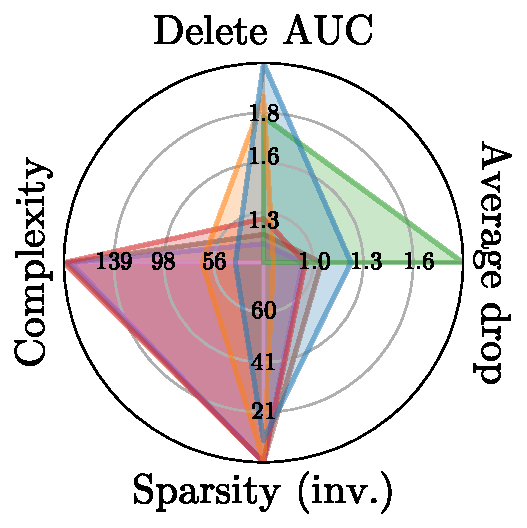
\includegraphics[scale=0.4]{./img/radar-flickr8k.pdf}
        \caption{Flickr8k}
    \end{subfigure}
    \begin{subfigure}[c]{0.26\linewidth}
        \centering
        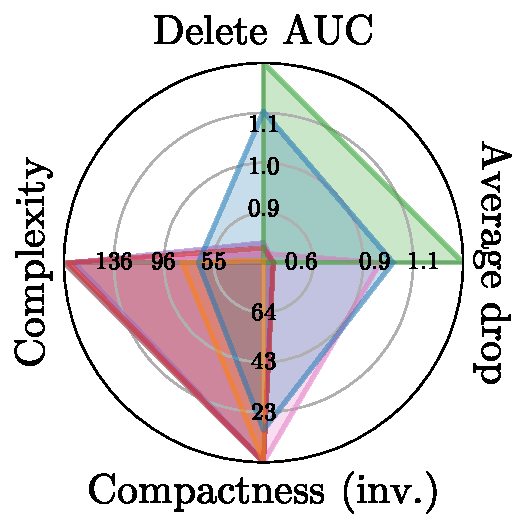
\includegraphics[scale=0.4]{./img/radar-hateful_memes.pdf}
        \caption{Hateful Memes}
    \end{subfigure}
    \begin{subfigure}[c]{0.26\linewidth}
        \centering
        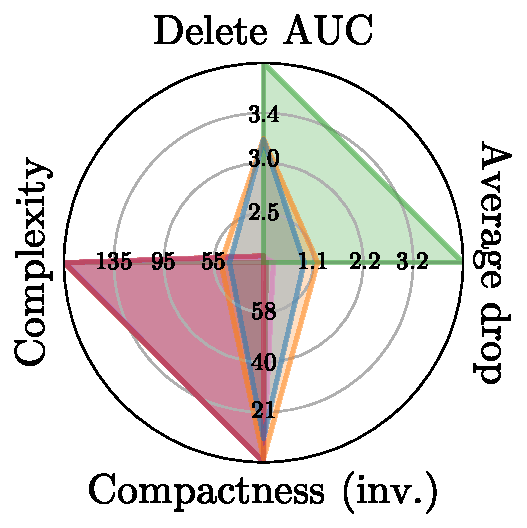
\includegraphics[scale=0.4]{./img/radar-snli_ve.pdf}
        \caption{SNLI-VE}
    \end{subfigure}
    \begin{subfigure}[c]{0.16\linewidth}
        \centering
        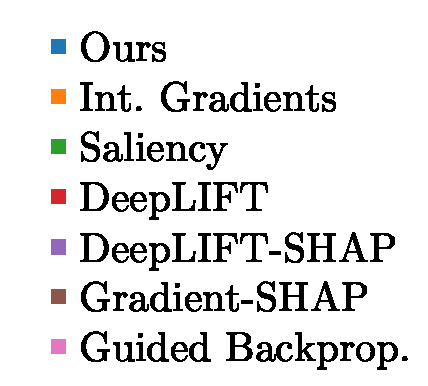
\includegraphics[scale=0.4]{./img/radar-legend.pdf}
    \end{subfigure}
    \caption{Radar plot of the quantitative metrics for the multimodal tasks. The closer to the center, the better.} \label{fig:radar_mm}
\end{figure}

For a qualitative evaluation, we analyze 100 samples from Flickr8k. We observed a consistent behavior as for text and image modality alone. The attribution maps that our method produces tend to be more well separated in terms of score magnitude, allowing to more clearly distinguish what is relevant. Also, as it does not lose in terms of faithfulness, what the scores give high relevance tend to usually be the object of interest in both the text sequence and figure. We provide a sample from the dataset in \Cref{fig:flickr8k_sample}.

\begin{figure}[t!]
    \centering
    \footnotesize
    \begin{subfigure}[b]{0.32\linewidth}
        \centering
        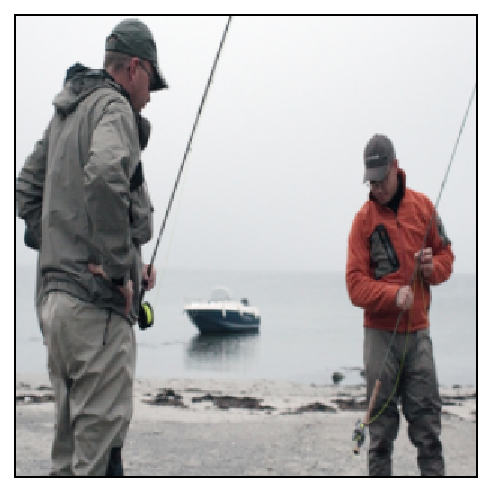
\includegraphics[width=0.8\linewidth]{./img/flickr8k.pdf}
    \end{subfigure}
    \begin{subfigure}[b]{0.32\linewidth}
        \centering
        \textbf{Ours} \\[-0.5em] {\scriptsize\tt\colorbox[RGB]{255, 247, 236}{\textcolor{black}{\vphantom{Tg}Men}} \colorbox[RGB]{127, 0, 0}{\textcolor{white}{\vphantom{Tg}standing}} \colorbox[RGB]{127, 0, 0}{\textcolor{white}{\vphantom{Tg}on}} \colorbox[RGB]{127, 0, 0}{\textcolor{white}{\vphantom{Tg}shore}} \colorbox[RGB]{127, 0, 0}{\textcolor{white}{\vphantom{Tg}with}} \colorbox[RGB]{127, 0, 0}{\textcolor{white}{\vphantom{Tg}fishing}} \colorbox[RGB]{127, 0, 0}{\textcolor{white}{\vphantom{Tg}pole}} \colorbox[RGB]{255, 247, 236}{\textcolor{black}{\vphantom{Tg}and}} \colorbox[RGB]{255, 247, 236}{\textcolor{black}{\vphantom{Tg}boat}} \colorbox[RGB]{255, 247, 236}{\textcolor{black}{\vphantom{Tg}in}} \colorbox[RGB]{252, 140, 89}{\textcolor{black}{\vphantom{Tg}water</s>}}}
        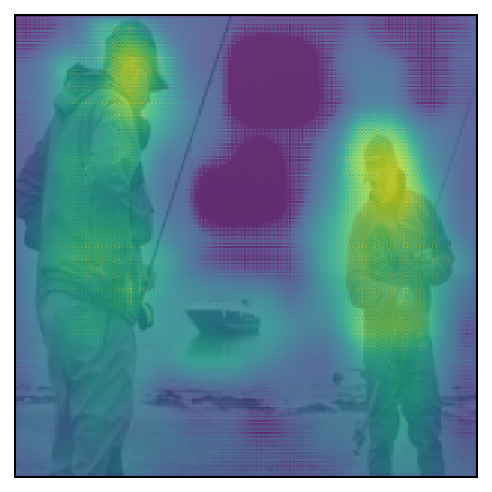
\includegraphics[width=0.8\linewidth]{./img/flickr8k-our.pdf}
    \end{subfigure}
    \begin{subfigure}[b]{0.32\linewidth}
        \centering
        \textbf{Saliency} \\[-0.5em] {\scriptsize\tt\colorbox[RGB]{253, 209, 155}{\textcolor{black}{\vphantom{Tg}Men}} \colorbox[RGB]{249, 130, 84}{\textcolor{black}{\vphantom{Tg}standing}} \colorbox[RGB]{252, 150, 98}{\textcolor{black}{\vphantom{Tg}on}} \colorbox[RGB]{253, 204, 150}{\textcolor{black}{\vphantom{Tg}shore}} \colorbox[RGB]{253, 218, 171}{\textcolor{black}{\vphantom{Tg}with}} \colorbox[RGB]{253, 179, 125}{\textcolor{black}{\vphantom{Tg}fishing}} \colorbox[RGB]{230, 82, 57}{\textcolor{black}{\vphantom{Tg}pole}} \colorbox[RGB]{127, 0, 0}{\textcolor{white}{\vphantom{Tg}and}} \colorbox[RGB]{250, 135, 87}{\textcolor{black}{\vphantom{Tg}boat}} \colorbox[RGB]{225, 70, 48}{\textcolor{black}{\vphantom{Tg}in}} \colorbox[RGB]{251, 138, 88}{\textcolor{black}{\vphantom{Tg}water</s>}}}\\
        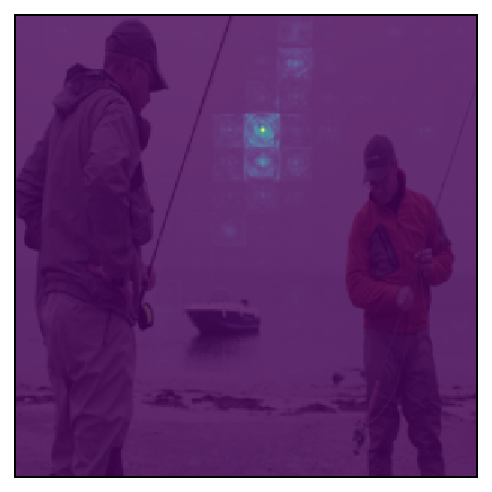
\includegraphics[width=0.8\linewidth]{./img/flickr8k-saliency.pdf}
    \end{subfigure}

    \vspace*{1em}
    
    \begin{subfigure}[b]{0.32\linewidth}
        \centering
        \textbf{Int. Gradients} \\[-0.5em] {\scriptsize\tt\colorbox[RGB]{253, 219, 172}{\textcolor{black}{\vphantom{Tg}Men}} \colorbox[RGB]{254, 223, 180}{\textcolor{black}{\vphantom{Tg}standing}} \colorbox[RGB]{254, 234, 204}{\textcolor{black}{\vphantom{Tg}on}} \colorbox[RGB]{253, 197, 142}{\textcolor{black}{\vphantom{Tg}shore}} \colorbox[RGB]{253, 175, 121}{\textcolor{black}{\vphantom{Tg}with}} \colorbox[RGB]{127, 0, 0}{\textcolor{white}{\vphantom{Tg}fishing}} \colorbox[RGB]{254, 239, 217}{\textcolor{black}{\vphantom{Tg}pole}} \colorbox[RGB]{253, 166, 113}{\textcolor{black}{\vphantom{Tg}and}} \colorbox[RGB]{249, 130, 84}{\textcolor{black}{\vphantom{Tg}boat}} \colorbox[RGB]{255, 247, 236}{\textcolor{black}{\vphantom{Tg}in}} \colorbox[RGB]{253, 166, 113}{\textcolor{black}{\vphantom{Tg}water</s>}}}\\
        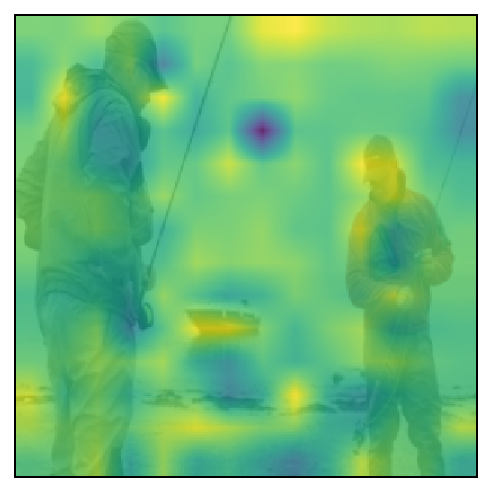
\includegraphics[width=0.8\linewidth]{./img/flickr8k-ig.pdf}
    \end{subfigure}
    \begin{subfigure}[b]{0.32\linewidth}
        \centering
        \textbf{DeepLIFT} \\[-0.5em] {\scriptsize\tt\colorbox[RGB]{233, 87, 61}{\textcolor{black}{\vphantom{Tg}Men}} \colorbox[RGB]{225, 70, 48}{\textcolor{black}{\vphantom{Tg}standing}} \colorbox[RGB]{205, 35, 22}{\textcolor{white}{\vphantom{Tg}on}} \colorbox[RGB]{218, 55, 36}{\textcolor{black}{\vphantom{Tg}shore}} \colorbox[RGB]{245, 120, 80}{\textcolor{black}{\vphantom{Tg}with}} \colorbox[RGB]{252, 162, 109}{\textcolor{black}{\vphantom{Tg}fishing}} \colorbox[RGB]{127, 0, 0}{\textcolor{white}{\vphantom{Tg}pole}} \colorbox[RGB]{223, 67, 45}{\textcolor{black}{\vphantom{Tg}and}} \colorbox[RGB]{255, 247, 236}{\textcolor{black}{\vphantom{Tg}boat}} \colorbox[RGB]{224, 68, 47}{\textcolor{black}{\vphantom{Tg}in}} \colorbox[RGB]{252, 140, 89}{\textcolor{black}{\vphantom{Tg}water</s>}}}\\
        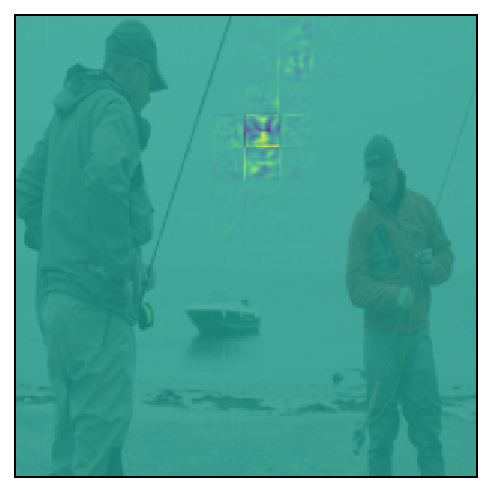
\includegraphics[width=0.8\linewidth]{./img/flickr8k-deeplift.pdf}
    \end{subfigure}
    \begin{subfigure}[b]{0.32\linewidth}
        \centering
        \textbf{DeepLIFT-SHAP} \\[-0.5em] {\scriptsize\tt\colorbox[RGB]{240, 105, 74}{\textcolor{black}{\vphantom{Tg}Men}} \colorbox[RGB]{244, 117, 79}{\textcolor{black}{\vphantom{Tg}standing}} \colorbox[RGB]{185, 8, 5}{\textcolor{white}{\vphantom{Tg}on}} \colorbox[RGB]{223, 65, 44}{\textcolor{black}{\vphantom{Tg}shore}} \colorbox[RGB]{244, 117, 79}{\textcolor{black}{\vphantom{Tg}with}} \colorbox[RGB]{253, 200, 146}{\textcolor{black}{\vphantom{Tg}fishing}} \colorbox[RGB]{127, 0, 0}{\textcolor{white}{\vphantom{Tg}pole}} \colorbox[RGB]{224, 68, 47}{\textcolor{black}{\vphantom{Tg}and}} \colorbox[RGB]{255, 247, 236}{\textcolor{black}{\vphantom{Tg}boat}} \colorbox[RGB]{143, 0, 0}{\textcolor{white}{\vphantom{Tg}in}} \colorbox[RGB]{252, 146, 94}{\textcolor{black}{\vphantom{Tg}water</s>}}}\\
        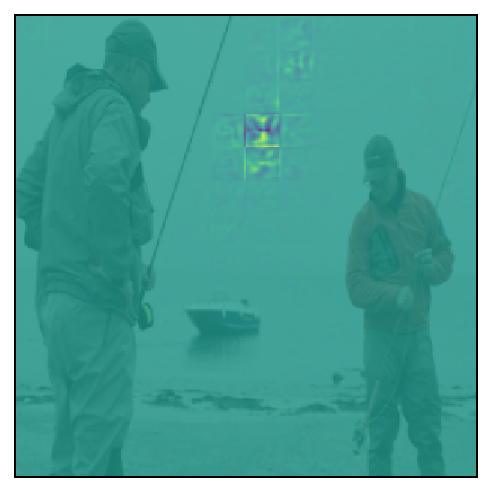
\includegraphics[width=0.8\linewidth]{./img/flickr8k-deepliftshap.pdf}
    \end{subfigure}

    \vspace*{1em}   

    \begin{subfigure}[b]{0.32\linewidth}
        \centering
        \textbf{Gradient-SHAP} \\[-0.5em] {\scriptsize\tt\colorbox[RGB]{252, 163, 110}{\textcolor{black}{\vphantom{Tg}Men}} \colorbox[RGB]{169, 0, 0}{\textcolor{white}{\vphantom{Tg}standing}} \colorbox[RGB]{127, 0, 0}{\textcolor{white}{\vphantom{Tg}on}} \colorbox[RGB]{216, 50, 33}{\textcolor{black}{\vphantom{Tg}shore}} \colorbox[RGB]{253, 194, 139}{\textcolor{black}{\vphantom{Tg}with}} \colorbox[RGB]{253, 184, 129}{\textcolor{black}{\vphantom{Tg}fishing}} \colorbox[RGB]{241, 106, 74}{\textcolor{black}{\vphantom{Tg}pole}} \colorbox[RGB]{254, 226, 188}{\textcolor{black}{\vphantom{Tg}and}} \colorbox[RGB]{252, 150, 98}{\textcolor{black}{\vphantom{Tg}boat}} \colorbox[RGB]{255, 247, 236}{\textcolor{black}{\vphantom{Tg}in}} \colorbox[RGB]{240, 103, 73}{\textcolor{black}{\vphantom{Tg}water</s>}}}\\
        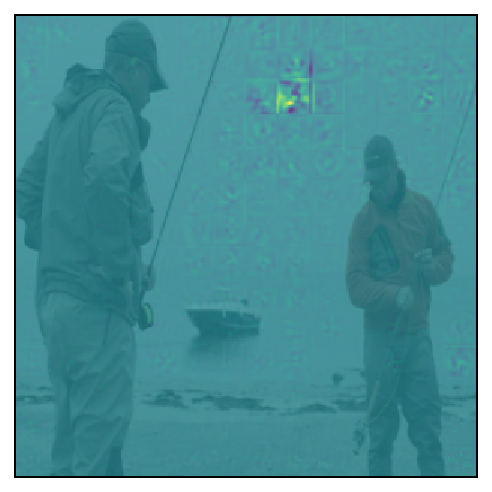
\includegraphics[width=0.8\linewidth]{./img/flickr8k-gradientshap.pdf}
    \end{subfigure}
    \begin{subfigure}[b]{0.32\linewidth}
        \centering
        \textbf{Guided backprop} \\[-0.5em] {\scriptsize\tt\colorbox[RGB]{254, 225, 185}{\textcolor{black}{\vphantom{Tg}Men}} \colorbox[RGB]{176, 0, 0}{\textcolor{white}{\vphantom{Tg}standing}} \colorbox[RGB]{250, 135, 87}{\textcolor{black}{\vphantom{Tg}on}} \colorbox[RGB]{254, 227, 189}{\textcolor{black}{\vphantom{Tg}shore}} \colorbox[RGB]{253, 195, 141}{\textcolor{black}{\vphantom{Tg}with}} \colorbox[RGB]{238, 98, 70}{\textcolor{black}{\vphantom{Tg}fishing}} \colorbox[RGB]{255, 247, 236}{\textcolor{black}{\vphantom{Tg}pole}} \colorbox[RGB]{127, 0, 0}{\textcolor{white}{\vphantom{Tg}and}} \colorbox[RGB]{240, 104, 73}{\textcolor{black}{\vphantom{Tg}boat}} \colorbox[RGB]{140, 0, 0}{\textcolor{white}{\vphantom{Tg}in}} \colorbox[RGB]{224, 68, 47}{\textcolor{black}{\vphantom{Tg}water</s>}}}\\
        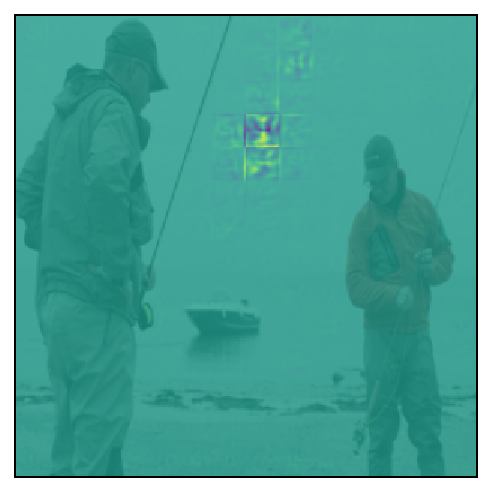
\includegraphics[width=0.8\linewidth]{./img/flickr8k-guidedbackprop.pdf}
    \end{subfigure}
    \caption{Sample from Flickr8k} \label{fig:flickr8k_sample}
\end{figure}

Overall, also in the case of multimodal classification, our method performs consistently by producing attribution maps with relatively low complexity and high sparsity while maintaining reasonable average drop and deletion AUC, highlighting again a good trade-off between visually appealing and faithful attribution maps compared to the other baselines that tend to favor only one side.



\section{Ablation Study}

To empirically experiment with the effectiveness of our design choices, we analyze the impact of the key components of our method. For computational efficiency, we limit ablation study to Tweet Sentiment Extraction and Imagenette to cover both modalities. We aim at testing whether the architectural choices and the training routine are effective. Therefore, we experiment with:
\begin{enumerate*}
    \item removing the last ReLU activation,
    \item removing the last sigmoid activation,
    \item removing the last rescaling step,
    \item removing the binary penalty in the loss,
    \item removing the magnitude penalty in the loss,
    \item removing the penalty in the loss completely,
    \item remove every component we introduce and train the model with only cross-entropy.
\end{enumerate*}

Results on Tweet Sentiment Extraction are presented in \Cref{tab:tweet_ablation} and a sample from the dataset is presented in \Cref{fig:tweet_ablation}. In terms of architecture, we can observe that, by either removing the final ReLU, sigmoid, or rescaling, there is a worsening in sparsity and an improvement in average drop and deletion AUC. This indicates, also as we can observe in \Cref{fig:tweet_ablation}, that the attribution maps becomes more expansive and considers more input tokens as relevant. Also in terms of loss function, we can observe that, after removing each component, results are decreased across all metrics. Finally, if everything is excluded, we can see that the method performs well in terms of average drop and deletion AUC, while it worsens in complexity and sparsity, indicating that the attribution map, without constraints, becomes trivially a non-informative result.


\begin{table}[t!]
    \centering
    \caption{Ablation results on Tweet Sentiment Extraction} \label{tab:tweet_ablation}
    \small
    \def\arraystretch{0.75}
    \makebox[\linewidth][c]{%
    \begin{tabular}{lcccc}
        \toprule
        \textbf{Method} & \textbf{Average drop $\downarrow$} & \textbf{Deletion AUC $\downarrow$} & \textbf{Complexity $\downarrow$} & \textbf{Sparsity $\uparrow$} \\
        \midrule
        Full              & 1.11 \std{1.52} & 1.61 \std{1.57} & 2.71 \std{1.04} & 87.21 \std{72.40} \\
        \midrule
        No ReLU           & 0.38 \std{0.58} & 0.66 \std{0.62} & 2.40 \std{0.68} & 81.95 \std{49.85} \\
        No sigmoid        & 1.28 \std{1.73} & 1.49 \std{1.63} & 3.04 \std{0.82} & 67.04 \std{53.80} \\
        No rescale        & 0.00 \std{0.01} & 0.17 \std{0.13} & 4.25 \std{0.96} & 32.32 \std{17.15} \\
        No binary pen.    & 1.26 \std{1.73} & 1.49 \std{1.69} & 3.16 \std{0.89} & 65.08 \std{53.13} \\
        No magnitude pen. & 1.29 \std{1.73} & 1.42 \std{1.68} & 3.35 \std{1.00} & 64.04 \std{53.90} \\
        No penalty        & 1.27 \std{1.73} & 1.40 \std{1.68} & 3.37 \std{1.02} & 63.76 \std{54.10} \\
        Nothing           & 0.06 \std{0.15} & 0.97 \std{0.77} & 3.19 \std{0.85} & 43.03 \std{26.78} \\
        \bottomrule
    \end{tabular}
    }
\end{table}

\begin{figure}[t!]
    \scriptsize
    \centering
    \makebox[\linewidth][c]{%
    \begin{tabular}{lc}
    \textbf{Full} & {\tt\colorbox[RGB]{127, 0, 0}{\textcolor{white}{\vphantom{Tg}I}} \colorbox[RGB]{127, 0, 0}{\textcolor{white}{\vphantom{Tg}want}} \colorbox[RGB]{255, 247, 236}{\textcolor{black}{\vphantom{Tg}cookies}} \colorbox[RGB]{255, 247, 236}{\textcolor{black}{\vphantom{Tg}for}} \colorbox[RGB]{252, 140, 89}{\textcolor{black}{\vphantom{Tg}breakfast!}} \colorbox[RGB]{255, 247, 236}{\textcolor{black}{\vphantom{Tg}Luckily}} \colorbox[RGB]{253, 195, 141}{\textcolor{black}{\vphantom{Tg}I`m}} \colorbox[RGB]{127, 0, 0}{\textcolor{white}{\vphantom{Tg}an}} \colorbox[RGB]{127, 0, 0}{\textcolor{white}{\vphantom{Tg}adult}} \colorbox[RGB]{255, 247, 236}{\textcolor{black}{\vphantom{Tg}and}} \colorbox[RGB]{127, 0, 0}{\textcolor{white}{\vphantom{Tg}can}} \colorbox[RGB]{127, 0, 0}{\textcolor{white}{\vphantom{Tg}do}} \colorbox[RGB]{231, 83, 58}{\textcolor{black}{\vphantom{Tg}that!</s>}}}\\
    \textbf{No ReLU} & {\tt\colorbox[RGB]{253, 215, 164}{\textcolor{black}{\vphantom{Tg}I}} \colorbox[RGB]{254, 237, 211}{\textcolor{black}{\vphantom{Tg}want}} \colorbox[RGB]{254, 239, 216}{\textcolor{black}{\vphantom{Tg}cookies}} \colorbox[RGB]{255, 247, 236}{\textcolor{black}{\vphantom{Tg}for}} \colorbox[RGB]{253, 184, 129}{\textcolor{black}{\vphantom{Tg}breakfast!}} \colorbox[RGB]{127, 0, 0}{\textcolor{white}{\vphantom{Tg}Luckily}} \colorbox[RGB]{253, 171, 117}{\textcolor{black}{\vphantom{Tg}I`m}} \colorbox[RGB]{253, 200, 146}{\textcolor{black}{\vphantom{Tg}an}} \colorbox[RGB]{253, 221, 177}{\textcolor{black}{\vphantom{Tg}adult}} \colorbox[RGB]{253, 176, 122}{\textcolor{black}{\vphantom{Tg}and}} \colorbox[RGB]{253, 192, 137}{\textcolor{black}{\vphantom{Tg}can}} \colorbox[RGB]{253, 217, 168}{\textcolor{black}{\vphantom{Tg}do}} \colorbox[RGB]{253, 197, 142}{\textcolor{black}{\vphantom{Tg}that!</s>}}}\\
    \textbf{No sigmoid} & {\tt\colorbox[RGB]{127, 0, 0}{\textcolor{white}{\vphantom{Tg}I}} \colorbox[RGB]{255, 247, 236}{\textcolor{black}{\vphantom{Tg}want}} \colorbox[RGB]{255, 247, 236}{\textcolor{black}{\vphantom{Tg}cookies}} \colorbox[RGB]{255, 247, 236}{\textcolor{black}{\vphantom{Tg}for}} \colorbox[RGB]{255, 247, 236}{\textcolor{black}{\vphantom{Tg}breakfast!}} \colorbox[RGB]{127, 0, 0}{\textcolor{white}{\vphantom{Tg}Luckily}} \colorbox[RGB]{231, 83, 58}{\textcolor{black}{\vphantom{Tg}I`m}} \colorbox[RGB]{127, 0, 0}{\textcolor{white}{\vphantom{Tg}an}} \colorbox[RGB]{127, 0, 0}{\textcolor{white}{\vphantom{Tg}adult}} \colorbox[RGB]{255, 247, 236}{\textcolor{black}{\vphantom{Tg}and}} \colorbox[RGB]{127, 0, 0}{\textcolor{white}{\vphantom{Tg}can}} \colorbox[RGB]{127, 0, 0}{\textcolor{white}{\vphantom{Tg}do}} \colorbox[RGB]{231, 83, 58}{\textcolor{black}{\vphantom{Tg}that!</s>}}}\\
    \textbf{No rescale} & {\tt\colorbox[RGB]{140, 0, 0}{\textcolor{white}{\vphantom{Tg}I}} \colorbox[RGB]{147, 0, 0}{\textcolor{white}{\vphantom{Tg}want}} \colorbox[RGB]{140, 0, 0}{\textcolor{white}{\vphantom{Tg}cookies}} \colorbox[RGB]{151, 0, 0}{\textcolor{white}{\vphantom{Tg}for}} \colorbox[RGB]{151, 0, 0}{\textcolor{white}{\vphantom{Tg}breakfast!}} \colorbox[RGB]{156, 0, 0}{\textcolor{white}{\vphantom{Tg}Luckily}} \colorbox[RGB]{148, 0, 0}{\textcolor{white}{\vphantom{Tg}I`m}} \colorbox[RGB]{148, 0, 0}{\textcolor{white}{\vphantom{Tg}an}} \colorbox[RGB]{134, 0, 0}{\textcolor{white}{\vphantom{Tg}adult}} \colorbox[RGB]{127, 0, 0}{\textcolor{white}{\vphantom{Tg}and}} \colorbox[RGB]{138, 0, 0}{\textcolor{white}{\vphantom{Tg}can}} \colorbox[RGB]{137, 0, 0}{\textcolor{white}{\vphantom{Tg}do}} \colorbox[RGB]{137, 0, 0}{\textcolor{white}{\vphantom{Tg}that!</s>}}}\\
    \textbf{No binary pen.} & {\tt\colorbox[RGB]{127, 0, 0}{\textcolor{white}{\vphantom{Tg}I}} \colorbox[RGB]{255, 247, 236}{\textcolor{black}{\vphantom{Tg}want}} \colorbox[RGB]{255, 247, 236}{\textcolor{black}{\vphantom{Tg}cookies}} \colorbox[RGB]{255, 247, 236}{\textcolor{black}{\vphantom{Tg}for}} \colorbox[RGB]{255, 247, 236}{\textcolor{black}{\vphantom{Tg}breakfast!}} \colorbox[RGB]{127, 0, 0}{\textcolor{white}{\vphantom{Tg}Luckily}} \colorbox[RGB]{231, 83, 58}{\textcolor{black}{\vphantom{Tg}I`m}} \colorbox[RGB]{127, 0, 0}{\textcolor{white}{\vphantom{Tg}an}} \colorbox[RGB]{127, 0, 0}{\textcolor{white}{\vphantom{Tg}adult}} \colorbox[RGB]{255, 247, 236}{\textcolor{black}{\vphantom{Tg}and}} \colorbox[RGB]{127, 0, 0}{\textcolor{white}{\vphantom{Tg}can}} \colorbox[RGB]{127, 0, 0}{\textcolor{white}{\vphantom{Tg}do}} \colorbox[RGB]{231, 83, 58}{\textcolor{black}{\vphantom{Tg}that!</s>}}}\\
    \textbf{No magnitude pen.} & {\tt\colorbox[RGB]{127, 0, 0}{\textcolor{white}{\vphantom{Tg}I}} \colorbox[RGB]{255, 247, 236}{\textcolor{black}{\vphantom{Tg}want}} \colorbox[RGB]{255, 247, 236}{\textcolor{black}{\vphantom{Tg}cookies}} \colorbox[RGB]{255, 247, 236}{\textcolor{black}{\vphantom{Tg}for}} \colorbox[RGB]{255, 247, 236}{\textcolor{black}{\vphantom{Tg}breakfast!}} \colorbox[RGB]{127, 0, 0}{\textcolor{white}{\vphantom{Tg}Luckily}} \colorbox[RGB]{231, 83, 58}{\textcolor{black}{\vphantom{Tg}I`m}} \colorbox[RGB]{127, 0, 0}{\textcolor{white}{\vphantom{Tg}an}} \colorbox[RGB]{127, 0, 0}{\textcolor{white}{\vphantom{Tg}adult}} \colorbox[RGB]{255, 247, 236}{\textcolor{black}{\vphantom{Tg}and}} \colorbox[RGB]{127, 0, 0}{\textcolor{white}{\vphantom{Tg}can}} \colorbox[RGB]{127, 0, 0}{\textcolor{white}{\vphantom{Tg}do}} \colorbox[RGB]{231, 83, 58}{\textcolor{black}{\vphantom{Tg}that!</s>}}}\\
    \textbf{No penalty} & {\tt\colorbox[RGB]{127, 0, 0}{\textcolor{white}{\vphantom{Tg}I}} \colorbox[RGB]{255, 247, 236}{\textcolor{black}{\vphantom{Tg}want}} \colorbox[RGB]{255, 247, 236}{\textcolor{black}{\vphantom{Tg}cookies}} \colorbox[RGB]{255, 247, 236}{\textcolor{black}{\vphantom{Tg}for}} \colorbox[RGB]{255, 247, 236}{\textcolor{black}{\vphantom{Tg}breakfast!}} \colorbox[RGB]{127, 0, 0}{\textcolor{white}{\vphantom{Tg}Luckily}} \colorbox[RGB]{231, 83, 58}{\textcolor{black}{\vphantom{Tg}I`m}} \colorbox[RGB]{127, 0, 0}{\textcolor{white}{\vphantom{Tg}an}} \colorbox[RGB]{127, 0, 0}{\textcolor{white}{\vphantom{Tg}adult}} \colorbox[RGB]{255, 247, 236}{\textcolor{black}{\vphantom{Tg}and}} \colorbox[RGB]{127, 0, 0}{\textcolor{white}{\vphantom{Tg}can}} \colorbox[RGB]{127, 0, 0}{\textcolor{white}{\vphantom{Tg}do}} \colorbox[RGB]{231, 83, 58}{\textcolor{black}{\vphantom{Tg}that!</s>}}}\\
    \textbf{Nothing} & {\tt\colorbox[RGB]{224, 68, 47}{\textcolor{black}{\vphantom{Tg}I}} \colorbox[RGB]{178, 0, 0}{\textcolor{white}{\vphantom{Tg}want}} \colorbox[RGB]{180, 2, 1}{\textcolor{white}{\vphantom{Tg}cookies}} \colorbox[RGB]{189, 14, 9}{\textcolor{white}{\vphantom{Tg}for}} \colorbox[RGB]{219, 57, 38}{\textcolor{black}{\vphantom{Tg}breakfast!}} \colorbox[RGB]{252, 142, 90}{\textcolor{black}{\vphantom{Tg}Luckily}} \colorbox[RGB]{227, 75, 52}{\textcolor{black}{\vphantom{Tg}I`m}} \colorbox[RGB]{226, 73, 51}{\textcolor{black}{\vphantom{Tg}an}} \colorbox[RGB]{211, 42, 27}{\textcolor{white}{\vphantom{Tg}adult}} \colorbox[RGB]{236, 95, 67}{\textcolor{black}{\vphantom{Tg}and}} \colorbox[RGB]{193, 18, 12}{\textcolor{white}{\vphantom{Tg}can}} \colorbox[RGB]{224, 68, 47}{\textcolor{black}{\vphantom{Tg}do}} \colorbox[RGB]{210, 41, 26}{\textcolor{white}{\vphantom{Tg}that!</s>}}}\\
    \end{tabular}
    }
    \caption{Ablation results on a sample from Tweet Sentiment Extraction} \label{fig:tweet_ablation}
\end{figure}


Ablation results on Imagenette are presented in \Cref{tab:imagenette_ablation} and a sample for qualitative analysis is shown in \Cref{fig:imagenette_ablation}. As for text, in all cases, but the scenario where rescaling is removed, performance on complexity and sparsity tend to worsen. In the case of rescaling, the behavior is opposite as average drop and deletion AUC worsen but complexity and sparsity improve. However, qualitatively we can see that the best result is obtained with every component as they allow to obtain a clearer distinction between what is relevant in the input.

\begin{table}[t!]
    \centering
    \caption{Ablation results on Imagenette} \label{tab:imagenette_ablation}
    \small
    \def\arraystretch{0.75}
    \makebox[\linewidth][c]{%
    \begin{tabular}{lcccc}
        \toprule
        \textbf{Method} & \textbf{Average drop $\downarrow$} & \textbf{Deletion AUC $\downarrow$} & \textbf{Complexity $\downarrow$} & \textbf{Sparsity $\uparrow$} \\
        \midrule
        Full               & 0.02 \std{0.07} & 0.27 \std{0.12} & 60.43  \std{19.45} & 7.02  \std{2.92} \\
        \midrule
        No ReLU            & 0.02 \std{0.06} & 0.30 \std{0.15} & 64.89  \std{18.82} & 4.74  \std{1.70} \\
        No sigmoid         & 0.02 \std{0.05} & 0.29 \std{0.12} & 60.31  \std{19.83} & 6.14  \std{2.82} \\
        No rescale         & 0.34 \std{0.26} & 0.45 \std{0.18} & 43.44  \std{46.93} & 22.03 \std{24.26} \\
        No binary pen.     & 0.02 \std{0.06} & 0.37 \std{0.09} & 48.68  \std{13.85} & 6.81  \std{3.45} \\
        No magnitude pen.  & 0.01 \std{0.03} & 0.04 \std{0.03} & 159.79 \std{25.34} & 1.92  \std{0.88} \\
        No penalty penalty & 0.01 \std{0.04} & 0.08 \std{0.07} & 149.04 \std{24.68} & 1.98  \std{0.78} \\
        Nothing            & 0.01 \std{0.02} & 0.06 \std{0.07} & 161.76 \std{30.60} & 1.56  \std{0.59} \\
        \bottomrule
    \end{tabular}
    }
\end{table}

\begin{figure}[t!]
    \centering
    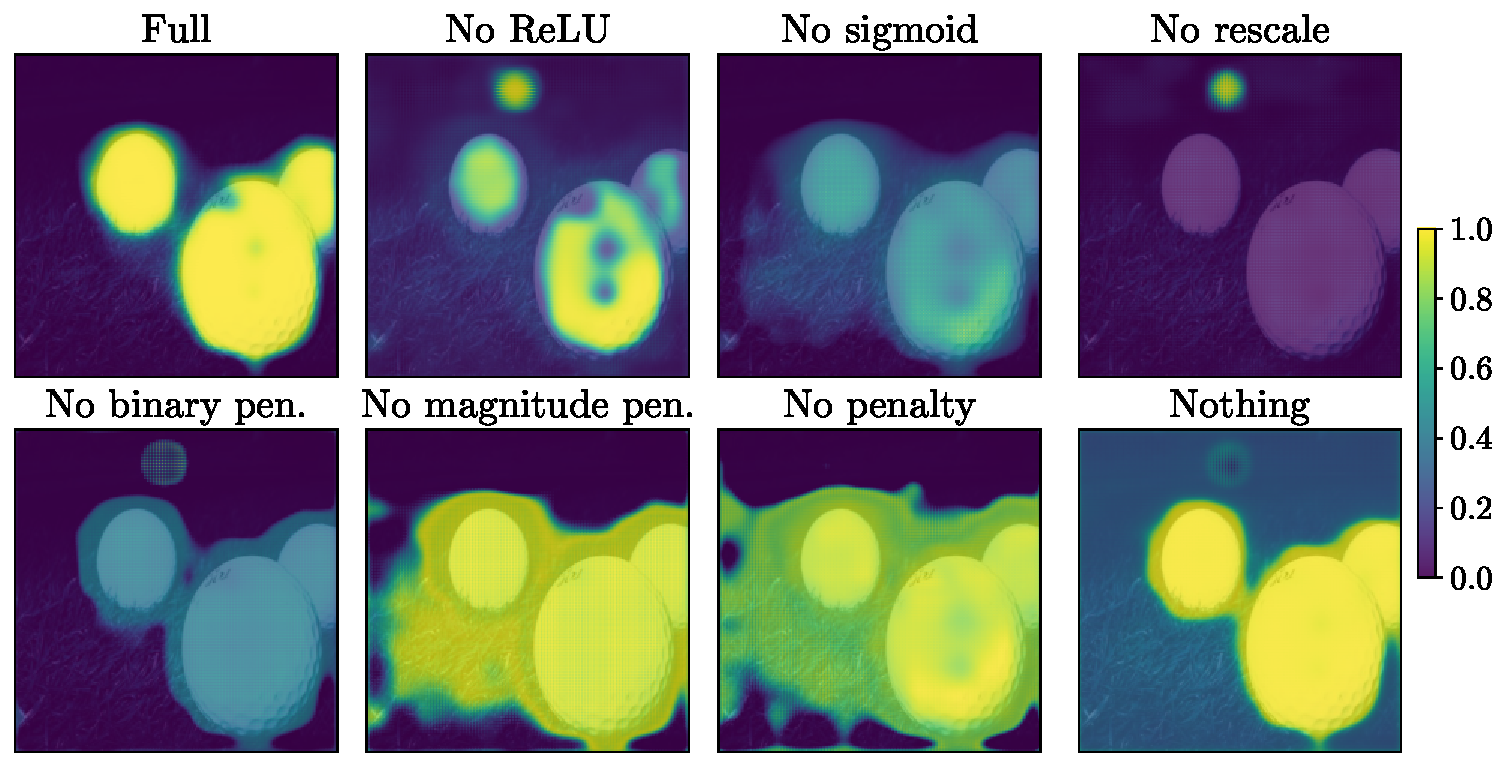
\includegraphics[width=0.9\linewidth]{./img/imagenette-ablation.pdf}
    \caption{Ablation results on a sample from Imagenette} \label{fig:imagenette_ablation}
\end{figure}
    \chapter{Conclusion} \label{ch:conclusion}

In this thesis, we presented a method for post-hoc explainability that produces attribution maps for the input space of neural networks. Our approach consists of training a dedicated neural network to produce attribution maps. With specific architectural and training choices, we developed a method that does not introduce new hyperparameters to tune other than those of a traditional neural network. After performing extensive quantitative and qualitative evaluation on classification datasets with text, image, and text-image modalities, we observed that our method produces attribution maps that are visually appealing while remaining faithful to the underlying model. Compared to other baselines, our method achieves the best trade-off between faithfulness, which we quantify as average drop and deletion AUC, and visual appeal, which we measure using complexity and compactness metrics, alongside a qualitative analysis. Future work can explore several directions: 
\begin{enumerate*}
    \item experiment with other modalities such as audio or time-series,
    \item apply the same approach on regression or generative tasks,
    \item explore other architectures for producing the attribution maps,
    \item perform more extensive experiments with larger datasets and with different domains.
\end{enumerate*}
    \cleardoublepage

    %%% Bibliography
    \pagestyle{plain}
    \printbibliography[heading=bibintoc]

    %%% Appendix
    % \cleardoublepage
    % \pagestyle{fancyAppendixContent}
    % \begin{appendices}
    %     \crefalias{chapter}{appendix}
    %     \include{chapters/appendix.tex}
    % \end{appendices}

\end{document}